\documentclass[11pt]{article}

    \usepackage[breakable]{tcolorbox}
    \usepackage{parskip} % Stop auto-indenting (to mimic markdown behaviour)
    
    \usepackage{iftex}
    \ifPDFTeX
    	\usepackage[T1]{fontenc}
    	\usepackage{mathpazo}
    \else
    	\usepackage{fontspec}
    \fi

    % Basic figure setup, for now with no caption control since it's done
    % automatically by Pandoc (which extracts ![](path) syntax from Markdown).
    \usepackage{graphicx}
    % Maintain compatibility with old templates. Remove in nbconvert 6.0
    \let\Oldincludegraphics\includegraphics
    % Ensure that by default, figures have no caption (until we provide a
    % proper Figure object with a Caption API and a way to capture that
    % in the conversion process - todo).
    \usepackage{caption}
    \DeclareCaptionFormat{nocaption}{}
    \captionsetup{format=nocaption,aboveskip=0pt,belowskip=0pt}

    \usepackage{float}
    \floatplacement{figure}{H} % forces figures to be placed at the correct location
    \usepackage{xcolor} % Allow colors to be defined
    \usepackage{enumerate} % Needed for markdown enumerations to work
    \usepackage{geometry} % Used to adjust the document margins
    \usepackage{amsmath} % Equations
    \usepackage{amssymb} % Equations
    \usepackage{textcomp} % defines textquotesingle
    % Hack from http://tex.stackexchange.com/a/47451/13684:
    \AtBeginDocument{%
        \def\PYZsq{\textquotesingle}% Upright quotes in Pygmentized code
    }
    \usepackage{upquote} % Upright quotes for verbatim code
    \usepackage{eurosym} % defines \euro
    \usepackage[mathletters]{ucs} % Extended unicode (utf-8) support
    \usepackage{fancyvrb} % verbatim replacement that allows latex
    \usepackage{grffile} % extends the file name processing of package graphics 
                         % to support a larger range
    \makeatletter % fix for old versions of grffile with XeLaTeX
    \@ifpackagelater{grffile}{2019/11/01}
    {
      % Do nothing on new versions
    }
    {
      \def\Gread@@xetex#1{%
        \IfFileExists{"\Gin@base".bb}%
        {\Gread@eps{\Gin@base.bb}}%
        {\Gread@@xetex@aux#1}%
      }
    }
    \makeatother
    \usepackage[Export]{adjustbox} % Used to constrain images to a maximum size
    \adjustboxset{max size={0.9\linewidth}{0.9\paperheight}}

    % The hyperref package gives us a pdf with properly built
    % internal navigation ('pdf bookmarks' for the table of contents,
    % internal cross-reference links, web links for URLs, etc.)
    \usepackage{hyperref}
    % The default LaTeX title has an obnoxious amount of whitespace. By default,
    % titling removes some of it. It also provides customization options.
    \usepackage{titling}
    \usepackage{longtable} % longtable support required by pandoc >1.10
    \usepackage{booktabs}  % table support for pandoc > 1.12.2
    \usepackage[inline]{enumitem} % IRkernel/repr support (it uses the enumerate* environment)
    \usepackage[normalem]{ulem} % ulem is needed to support strikethroughs (\sout)
                                % normalem makes italics be italics, not underlines
    \usepackage{mathrsfs}
    

    
    % Colors for the hyperref package
    \definecolor{urlcolor}{rgb}{0,.145,.698}
    \definecolor{linkcolor}{rgb}{.71,0.21,0.01}
    \definecolor{citecolor}{rgb}{.12,.54,.11}

    % ANSI colors
    \definecolor{ansi-black}{HTML}{3E424D}
    \definecolor{ansi-black-intense}{HTML}{282C36}
    \definecolor{ansi-red}{HTML}{E75C58}
    \definecolor{ansi-red-intense}{HTML}{B22B31}
    \definecolor{ansi-green}{HTML}{00A250}
    \definecolor{ansi-green-intense}{HTML}{007427}
    \definecolor{ansi-yellow}{HTML}{DDB62B}
    \definecolor{ansi-yellow-intense}{HTML}{B27D12}
    \definecolor{ansi-blue}{HTML}{208FFB}
    \definecolor{ansi-blue-intense}{HTML}{0065CA}
    \definecolor{ansi-magenta}{HTML}{D160C4}
    \definecolor{ansi-magenta-intense}{HTML}{A03196}
    \definecolor{ansi-cyan}{HTML}{60C6C8}
    \definecolor{ansi-cyan-intense}{HTML}{258F8F}
    \definecolor{ansi-white}{HTML}{C5C1B4}
    \definecolor{ansi-white-intense}{HTML}{A1A6B2}
    \definecolor{ansi-default-inverse-fg}{HTML}{FFFFFF}
    \definecolor{ansi-default-inverse-bg}{HTML}{000000}

    % common color for the border for error outputs.
    \definecolor{outerrorbackground}{HTML}{FFDFDF}

    % commands and environments needed by pandoc snippets
    % extracted from the output of `pandoc -s`
    \providecommand{\tightlist}{%
      \setlength{\itemsep}{0pt}\setlength{\parskip}{0pt}}
    \DefineVerbatimEnvironment{Highlighting}{Verbatim}{commandchars=\\\{\}}
    % Add ',fontsize=\small' for more characters per line
    \newenvironment{Shaded}{}{}
    \newcommand{\KeywordTok}[1]{\textcolor[rgb]{0.00,0.44,0.13}{\textbf{{#1}}}}
    \newcommand{\DataTypeTok}[1]{\textcolor[rgb]{0.56,0.13,0.00}{{#1}}}
    \newcommand{\DecValTok}[1]{\textcolor[rgb]{0.25,0.63,0.44}{{#1}}}
    \newcommand{\BaseNTok}[1]{\textcolor[rgb]{0.25,0.63,0.44}{{#1}}}
    \newcommand{\FloatTok}[1]{\textcolor[rgb]{0.25,0.63,0.44}{{#1}}}
    \newcommand{\CharTok}[1]{\textcolor[rgb]{0.25,0.44,0.63}{{#1}}}
    \newcommand{\StringTok}[1]{\textcolor[rgb]{0.25,0.44,0.63}{{#1}}}
    \newcommand{\CommentTok}[1]{\textcolor[rgb]{0.38,0.63,0.69}{\textit{{#1}}}}
    \newcommand{\OtherTok}[1]{\textcolor[rgb]{0.00,0.44,0.13}{{#1}}}
    \newcommand{\AlertTok}[1]{\textcolor[rgb]{1.00,0.00,0.00}{\textbf{{#1}}}}
    \newcommand{\FunctionTok}[1]{\textcolor[rgb]{0.02,0.16,0.49}{{#1}}}
    \newcommand{\RegionMarkerTok}[1]{{#1}}
    \newcommand{\ErrorTok}[1]{\textcolor[rgb]{1.00,0.00,0.00}{\textbf{{#1}}}}
    \newcommand{\NormalTok}[1]{{#1}}
    
    % Additional commands for more recent versions of Pandoc
    \newcommand{\ConstantTok}[1]{\textcolor[rgb]{0.53,0.00,0.00}{{#1}}}
    \newcommand{\SpecialCharTok}[1]{\textcolor[rgb]{0.25,0.44,0.63}{{#1}}}
    \newcommand{\VerbatimStringTok}[1]{\textcolor[rgb]{0.25,0.44,0.63}{{#1}}}
    \newcommand{\SpecialStringTok}[1]{\textcolor[rgb]{0.73,0.40,0.53}{{#1}}}
    \newcommand{\ImportTok}[1]{{#1}}
    \newcommand{\DocumentationTok}[1]{\textcolor[rgb]{0.73,0.13,0.13}{\textit{{#1}}}}
    \newcommand{\AnnotationTok}[1]{\textcolor[rgb]{0.38,0.63,0.69}{\textbf{\textit{{#1}}}}}
    \newcommand{\CommentVarTok}[1]{\textcolor[rgb]{0.38,0.63,0.69}{\textbf{\textit{{#1}}}}}
    \newcommand{\VariableTok}[1]{\textcolor[rgb]{0.10,0.09,0.49}{{#1}}}
    \newcommand{\ControlFlowTok}[1]{\textcolor[rgb]{0.00,0.44,0.13}{\textbf{{#1}}}}
    \newcommand{\OperatorTok}[1]{\textcolor[rgb]{0.40,0.40,0.40}{{#1}}}
    \newcommand{\BuiltInTok}[1]{{#1}}
    \newcommand{\ExtensionTok}[1]{{#1}}
    \newcommand{\PreprocessorTok}[1]{\textcolor[rgb]{0.74,0.48,0.00}{{#1}}}
    \newcommand{\AttributeTok}[1]{\textcolor[rgb]{0.49,0.56,0.16}{{#1}}}
    \newcommand{\InformationTok}[1]{\textcolor[rgb]{0.38,0.63,0.69}{\textbf{\textit{{#1}}}}}
    \newcommand{\WarningTok}[1]{\textcolor[rgb]{0.38,0.63,0.69}{\textbf{\textit{{#1}}}}}
    
    
    % Define a nice break command that doesn't care if a line doesn't already
    % exist.
    \def\br{\hspace*{\fill} \\* }
    % Math Jax compatibility definitions
    \def\gt{>}
    \def\lt{<}
    \let\Oldtex\TeX
    \let\Oldlatex\LaTeX
    \renewcommand{\TeX}{\textrm{\Oldtex}}
    \renewcommand{\LaTeX}{\textrm{\Oldlatex}}
    % Document parameters
    % Document title
    \title{the-promise-to-partner}
    
    
    
    
    
% Pygments definitions
\makeatletter
\def\PY@reset{\let\PY@it=\relax \let\PY@bf=\relax%
    \let\PY@ul=\relax \let\PY@tc=\relax%
    \let\PY@bc=\relax \let\PY@ff=\relax}
\def\PY@tok#1{\csname PY@tok@#1\endcsname}
\def\PY@toks#1+{\ifx\relax#1\empty\else%
    \PY@tok{#1}\expandafter\PY@toks\fi}
\def\PY@do#1{\PY@bc{\PY@tc{\PY@ul{%
    \PY@it{\PY@bf{\PY@ff{#1}}}}}}}
\def\PY#1#2{\PY@reset\PY@toks#1+\relax+\PY@do{#2}}

\@namedef{PY@tok@w}{\def\PY@tc##1{\textcolor[rgb]{0.73,0.73,0.73}{##1}}}
\@namedef{PY@tok@c}{\let\PY@it=\textit\def\PY@tc##1{\textcolor[rgb]{0.25,0.50,0.50}{##1}}}
\@namedef{PY@tok@cp}{\def\PY@tc##1{\textcolor[rgb]{0.74,0.48,0.00}{##1}}}
\@namedef{PY@tok@k}{\let\PY@bf=\textbf\def\PY@tc##1{\textcolor[rgb]{0.00,0.50,0.00}{##1}}}
\@namedef{PY@tok@kp}{\def\PY@tc##1{\textcolor[rgb]{0.00,0.50,0.00}{##1}}}
\@namedef{PY@tok@kt}{\def\PY@tc##1{\textcolor[rgb]{0.69,0.00,0.25}{##1}}}
\@namedef{PY@tok@o}{\def\PY@tc##1{\textcolor[rgb]{0.40,0.40,0.40}{##1}}}
\@namedef{PY@tok@ow}{\let\PY@bf=\textbf\def\PY@tc##1{\textcolor[rgb]{0.67,0.13,1.00}{##1}}}
\@namedef{PY@tok@nb}{\def\PY@tc##1{\textcolor[rgb]{0.00,0.50,0.00}{##1}}}
\@namedef{PY@tok@nf}{\def\PY@tc##1{\textcolor[rgb]{0.00,0.00,1.00}{##1}}}
\@namedef{PY@tok@nc}{\let\PY@bf=\textbf\def\PY@tc##1{\textcolor[rgb]{0.00,0.00,1.00}{##1}}}
\@namedef{PY@tok@nn}{\let\PY@bf=\textbf\def\PY@tc##1{\textcolor[rgb]{0.00,0.00,1.00}{##1}}}
\@namedef{PY@tok@ne}{\let\PY@bf=\textbf\def\PY@tc##1{\textcolor[rgb]{0.82,0.25,0.23}{##1}}}
\@namedef{PY@tok@nv}{\def\PY@tc##1{\textcolor[rgb]{0.10,0.09,0.49}{##1}}}
\@namedef{PY@tok@no}{\def\PY@tc##1{\textcolor[rgb]{0.53,0.00,0.00}{##1}}}
\@namedef{PY@tok@nl}{\def\PY@tc##1{\textcolor[rgb]{0.63,0.63,0.00}{##1}}}
\@namedef{PY@tok@ni}{\let\PY@bf=\textbf\def\PY@tc##1{\textcolor[rgb]{0.60,0.60,0.60}{##1}}}
\@namedef{PY@tok@na}{\def\PY@tc##1{\textcolor[rgb]{0.49,0.56,0.16}{##1}}}
\@namedef{PY@tok@nt}{\let\PY@bf=\textbf\def\PY@tc##1{\textcolor[rgb]{0.00,0.50,0.00}{##1}}}
\@namedef{PY@tok@nd}{\def\PY@tc##1{\textcolor[rgb]{0.67,0.13,1.00}{##1}}}
\@namedef{PY@tok@s}{\def\PY@tc##1{\textcolor[rgb]{0.73,0.13,0.13}{##1}}}
\@namedef{PY@tok@sd}{\let\PY@it=\textit\def\PY@tc##1{\textcolor[rgb]{0.73,0.13,0.13}{##1}}}
\@namedef{PY@tok@si}{\let\PY@bf=\textbf\def\PY@tc##1{\textcolor[rgb]{0.73,0.40,0.53}{##1}}}
\@namedef{PY@tok@se}{\let\PY@bf=\textbf\def\PY@tc##1{\textcolor[rgb]{0.73,0.40,0.13}{##1}}}
\@namedef{PY@tok@sr}{\def\PY@tc##1{\textcolor[rgb]{0.73,0.40,0.53}{##1}}}
\@namedef{PY@tok@ss}{\def\PY@tc##1{\textcolor[rgb]{0.10,0.09,0.49}{##1}}}
\@namedef{PY@tok@sx}{\def\PY@tc##1{\textcolor[rgb]{0.00,0.50,0.00}{##1}}}
\@namedef{PY@tok@m}{\def\PY@tc##1{\textcolor[rgb]{0.40,0.40,0.40}{##1}}}
\@namedef{PY@tok@gh}{\let\PY@bf=\textbf\def\PY@tc##1{\textcolor[rgb]{0.00,0.00,0.50}{##1}}}
\@namedef{PY@tok@gu}{\let\PY@bf=\textbf\def\PY@tc##1{\textcolor[rgb]{0.50,0.00,0.50}{##1}}}
\@namedef{PY@tok@gd}{\def\PY@tc##1{\textcolor[rgb]{0.63,0.00,0.00}{##1}}}
\@namedef{PY@tok@gi}{\def\PY@tc##1{\textcolor[rgb]{0.00,0.63,0.00}{##1}}}
\@namedef{PY@tok@gr}{\def\PY@tc##1{\textcolor[rgb]{1.00,0.00,0.00}{##1}}}
\@namedef{PY@tok@ge}{\let\PY@it=\textit}
\@namedef{PY@tok@gs}{\let\PY@bf=\textbf}
\@namedef{PY@tok@gp}{\let\PY@bf=\textbf\def\PY@tc##1{\textcolor[rgb]{0.00,0.00,0.50}{##1}}}
\@namedef{PY@tok@go}{\def\PY@tc##1{\textcolor[rgb]{0.53,0.53,0.53}{##1}}}
\@namedef{PY@tok@gt}{\def\PY@tc##1{\textcolor[rgb]{0.00,0.27,0.87}{##1}}}
\@namedef{PY@tok@err}{\def\PY@bc##1{{\setlength{\fboxsep}{\string -\fboxrule}\fcolorbox[rgb]{1.00,0.00,0.00}{1,1,1}{\strut ##1}}}}
\@namedef{PY@tok@kc}{\let\PY@bf=\textbf\def\PY@tc##1{\textcolor[rgb]{0.00,0.50,0.00}{##1}}}
\@namedef{PY@tok@kd}{\let\PY@bf=\textbf\def\PY@tc##1{\textcolor[rgb]{0.00,0.50,0.00}{##1}}}
\@namedef{PY@tok@kn}{\let\PY@bf=\textbf\def\PY@tc##1{\textcolor[rgb]{0.00,0.50,0.00}{##1}}}
\@namedef{PY@tok@kr}{\let\PY@bf=\textbf\def\PY@tc##1{\textcolor[rgb]{0.00,0.50,0.00}{##1}}}
\@namedef{PY@tok@bp}{\def\PY@tc##1{\textcolor[rgb]{0.00,0.50,0.00}{##1}}}
\@namedef{PY@tok@fm}{\def\PY@tc##1{\textcolor[rgb]{0.00,0.00,1.00}{##1}}}
\@namedef{PY@tok@vc}{\def\PY@tc##1{\textcolor[rgb]{0.10,0.09,0.49}{##1}}}
\@namedef{PY@tok@vg}{\def\PY@tc##1{\textcolor[rgb]{0.10,0.09,0.49}{##1}}}
\@namedef{PY@tok@vi}{\def\PY@tc##1{\textcolor[rgb]{0.10,0.09,0.49}{##1}}}
\@namedef{PY@tok@vm}{\def\PY@tc##1{\textcolor[rgb]{0.10,0.09,0.49}{##1}}}
\@namedef{PY@tok@sa}{\def\PY@tc##1{\textcolor[rgb]{0.73,0.13,0.13}{##1}}}
\@namedef{PY@tok@sb}{\def\PY@tc##1{\textcolor[rgb]{0.73,0.13,0.13}{##1}}}
\@namedef{PY@tok@sc}{\def\PY@tc##1{\textcolor[rgb]{0.73,0.13,0.13}{##1}}}
\@namedef{PY@tok@dl}{\def\PY@tc##1{\textcolor[rgb]{0.73,0.13,0.13}{##1}}}
\@namedef{PY@tok@s2}{\def\PY@tc##1{\textcolor[rgb]{0.73,0.13,0.13}{##1}}}
\@namedef{PY@tok@sh}{\def\PY@tc##1{\textcolor[rgb]{0.73,0.13,0.13}{##1}}}
\@namedef{PY@tok@s1}{\def\PY@tc##1{\textcolor[rgb]{0.73,0.13,0.13}{##1}}}
\@namedef{PY@tok@mb}{\def\PY@tc##1{\textcolor[rgb]{0.40,0.40,0.40}{##1}}}
\@namedef{PY@tok@mf}{\def\PY@tc##1{\textcolor[rgb]{0.40,0.40,0.40}{##1}}}
\@namedef{PY@tok@mh}{\def\PY@tc##1{\textcolor[rgb]{0.40,0.40,0.40}{##1}}}
\@namedef{PY@tok@mi}{\def\PY@tc##1{\textcolor[rgb]{0.40,0.40,0.40}{##1}}}
\@namedef{PY@tok@il}{\def\PY@tc##1{\textcolor[rgb]{0.40,0.40,0.40}{##1}}}
\@namedef{PY@tok@mo}{\def\PY@tc##1{\textcolor[rgb]{0.40,0.40,0.40}{##1}}}
\@namedef{PY@tok@ch}{\let\PY@it=\textit\def\PY@tc##1{\textcolor[rgb]{0.25,0.50,0.50}{##1}}}
\@namedef{PY@tok@cm}{\let\PY@it=\textit\def\PY@tc##1{\textcolor[rgb]{0.25,0.50,0.50}{##1}}}
\@namedef{PY@tok@cpf}{\let\PY@it=\textit\def\PY@tc##1{\textcolor[rgb]{0.25,0.50,0.50}{##1}}}
\@namedef{PY@tok@c1}{\let\PY@it=\textit\def\PY@tc##1{\textcolor[rgb]{0.25,0.50,0.50}{##1}}}
\@namedef{PY@tok@cs}{\let\PY@it=\textit\def\PY@tc##1{\textcolor[rgb]{0.25,0.50,0.50}{##1}}}

\def\PYZbs{\char`\\}
\def\PYZus{\char`\_}
\def\PYZob{\char`\{}
\def\PYZcb{\char`\}}
\def\PYZca{\char`\^}
\def\PYZam{\char`\&}
\def\PYZlt{\char`\<}
\def\PYZgt{\char`\>}
\def\PYZsh{\char`\#}
\def\PYZpc{\char`\%}
\def\PYZdl{\char`\$}
\def\PYZhy{\char`\-}
\def\PYZsq{\char`\'}
\def\PYZdq{\char`\"}
\def\PYZti{\char`\~}
% for compatibility with earlier versions
\def\PYZat{@}
\def\PYZlb{[}
\def\PYZrb{]}
\makeatother


    % For linebreaks inside Verbatim environment from package fancyvrb. 
    \makeatletter
        \newbox\Wrappedcontinuationbox 
        \newbox\Wrappedvisiblespacebox 
        \newcommand*\Wrappedvisiblespace {\textcolor{red}{\textvisiblespace}} 
        \newcommand*\Wrappedcontinuationsymbol {\textcolor{red}{\llap{\tiny$\m@th\hookrightarrow$}}} 
        \newcommand*\Wrappedcontinuationindent {3ex } 
        \newcommand*\Wrappedafterbreak {\kern\Wrappedcontinuationindent\copy\Wrappedcontinuationbox} 
        % Take advantage of the already applied Pygments mark-up to insert 
        % potential linebreaks for TeX processing. 
        %        {, <, #, %, $, ' and ": go to next line. 
        %        _, }, ^, &, >, - and ~: stay at end of broken line. 
        % Use of \textquotesingle for straight quote. 
        \newcommand*\Wrappedbreaksatspecials {% 
            \def\PYGZus{\discretionary{\char`\_}{\Wrappedafterbreak}{\char`\_}}% 
            \def\PYGZob{\discretionary{}{\Wrappedafterbreak\char`\{}{\char`\{}}% 
            \def\PYGZcb{\discretionary{\char`\}}{\Wrappedafterbreak}{\char`\}}}% 
            \def\PYGZca{\discretionary{\char`\^}{\Wrappedafterbreak}{\char`\^}}% 
            \def\PYGZam{\discretionary{\char`\&}{\Wrappedafterbreak}{\char`\&}}% 
            \def\PYGZlt{\discretionary{}{\Wrappedafterbreak\char`\<}{\char`\<}}% 
            \def\PYGZgt{\discretionary{\char`\>}{\Wrappedafterbreak}{\char`\>}}% 
            \def\PYGZsh{\discretionary{}{\Wrappedafterbreak\char`\#}{\char`\#}}% 
            \def\PYGZpc{\discretionary{}{\Wrappedafterbreak\char`\%}{\char`\%}}% 
            \def\PYGZdl{\discretionary{}{\Wrappedafterbreak\char`\$}{\char`\$}}% 
            \def\PYGZhy{\discretionary{\char`\-}{\Wrappedafterbreak}{\char`\-}}% 
            \def\PYGZsq{\discretionary{}{\Wrappedafterbreak\textquotesingle}{\textquotesingle}}% 
            \def\PYGZdq{\discretionary{}{\Wrappedafterbreak\char`\"}{\char`\"}}% 
            \def\PYGZti{\discretionary{\char`\~}{\Wrappedafterbreak}{\char`\~}}% 
        } 
        % Some characters . , ; ? ! / are not pygmentized. 
        % This macro makes them "active" and they will insert potential linebreaks 
        \newcommand*\Wrappedbreaksatpunct {% 
            \lccode`\~`\.\lowercase{\def~}{\discretionary{\hbox{\char`\.}}{\Wrappedafterbreak}{\hbox{\char`\.}}}% 
            \lccode`\~`\,\lowercase{\def~}{\discretionary{\hbox{\char`\,}}{\Wrappedafterbreak}{\hbox{\char`\,}}}% 
            \lccode`\~`\;\lowercase{\def~}{\discretionary{\hbox{\char`\;}}{\Wrappedafterbreak}{\hbox{\char`\;}}}% 
            \lccode`\~`\:\lowercase{\def~}{\discretionary{\hbox{\char`\:}}{\Wrappedafterbreak}{\hbox{\char`\:}}}% 
            \lccode`\~`\?\lowercase{\def~}{\discretionary{\hbox{\char`\?}}{\Wrappedafterbreak}{\hbox{\char`\?}}}% 
            \lccode`\~`\!\lowercase{\def~}{\discretionary{\hbox{\char`\!}}{\Wrappedafterbreak}{\hbox{\char`\!}}}% 
            \lccode`\~`\/\lowercase{\def~}{\discretionary{\hbox{\char`\/}}{\Wrappedafterbreak}{\hbox{\char`\/}}}% 
            \catcode`\.\active
            \catcode`\,\active 
            \catcode`\;\active
            \catcode`\:\active
            \catcode`\?\active
            \catcode`\!\active
            \catcode`\/\active 
            \lccode`\~`\~ 	
        }
    \makeatother

    \let\OriginalVerbatim=\Verbatim
    \makeatletter
    \renewcommand{\Verbatim}[1][1]{%
        %\parskip\z@skip
        \sbox\Wrappedcontinuationbox {\Wrappedcontinuationsymbol}%
        \sbox\Wrappedvisiblespacebox {\FV@SetupFont\Wrappedvisiblespace}%
        \def\FancyVerbFormatLine ##1{\hsize\linewidth
            \vtop{\raggedright\hyphenpenalty\z@\exhyphenpenalty\z@
                \doublehyphendemerits\z@\finalhyphendemerits\z@
                \strut ##1\strut}%
        }%
        % If the linebreak is at a space, the latter will be displayed as visible
        % space at end of first line, and a continuation symbol starts next line.
        % Stretch/shrink are however usually zero for typewriter font.
        \def\FV@Space {%
            \nobreak\hskip\z@ plus\fontdimen3\font minus\fontdimen4\font
            \discretionary{\copy\Wrappedvisiblespacebox}{\Wrappedafterbreak}
            {\kern\fontdimen2\font}%
        }%
        
        % Allow breaks at special characters using \PYG... macros.
        \Wrappedbreaksatspecials
        % Breaks at punctuation characters . , ; ? ! and / need catcode=\active 	
        \OriginalVerbatim[#1,codes*=\Wrappedbreaksatpunct]%
    }
    \makeatother

    % Exact colors from NB
    \definecolor{incolor}{HTML}{303F9F}
    \definecolor{outcolor}{HTML}{D84315}
    \definecolor{cellborder}{HTML}{CFCFCF}
    \definecolor{cellbackground}{HTML}{F7F7F7}
    
    % prompt
    \makeatletter
    \newcommand{\boxspacing}{\kern\kvtcb@left@rule\kern\kvtcb@boxsep}
    \makeatother
    \newcommand{\prompt}[4]{
        {\ttfamily\llap{{\color{#2}[#3]:\hspace{3pt}#4}}\vspace{-\baselineskip}}
    }
    

    
    % Prevent overflowing lines due to hard-to-break entities
    \sloppy 
    % Setup hyperref package
    \hypersetup{
      breaklinks=true,  % so long urls are correctly broken across lines
      colorlinks=true,
      urlcolor=urlcolor,
      linkcolor=linkcolor,
      citecolor=citecolor,
      }
    % Slightly bigger margins than the latex defaults
    
    \geometry{verbose,tmargin=1in,bmargin=1in,lmargin=1in,rmargin=1in}
    
    

\begin{document}
    
    \maketitle
    
    

    
    \hypertarget{the-promise-to-partner}{%
\section{The Promise to Partner}\label{the-promise-to-partner}}

    In this JupyterNotebook we show you how to visualize and analyze a
network. We do this using the example of the consortia that are
participating in or have applied to the National Research Data
Infrastructure Initiative (NFDI).

As a data basis, we take the \emph{Letters of Intent} of the respective
consortia, in which cooperation partners are named. These mentions are
the starting point of our network\footnote{See also the repository of
  Dorothea Strecker (https://github.com/dorothearrr/NFDI\_Netzwerk),
  where she has already done a similar visualization and analysis.}.

We do the visualization in a JupyterNotebook or R Notebook\footnote{https://rnotebook.io
  cf.~https://bookdown.org/yihui/rmarkdown/notebook.html}, so no local
installation of R is necessary. JupyterNotebooks are built in such a way
that you have different cells in which you write code (in our case
\texttt{R} code). To run the cell with the code, we can click on
``\emph{Cell}'' and ``\emph{Run Cells}'' in the menu. Or click with the
cursor in the cell and then press \emph{SHIFT}'' and ``\emph{ENTER}'' at
the same time. You will then see the result of the code displayed
directly below the cell.

    Before we get started, let's clarify a few terms. A network consists of
two components:

\begin{itemize}
\tightlist
\item
  Nodes (circle)
\item
  Edges (line)
\end{itemize}

Nodes (\emph{nodes} or \emph{vertices}) are represented as circles and
represent consortia. Edges (\emph{edges}) are represented as more or
less curved lines and emanate from the nodes. They indicate a connection
between two nodes.

\begin{figure}
\centering
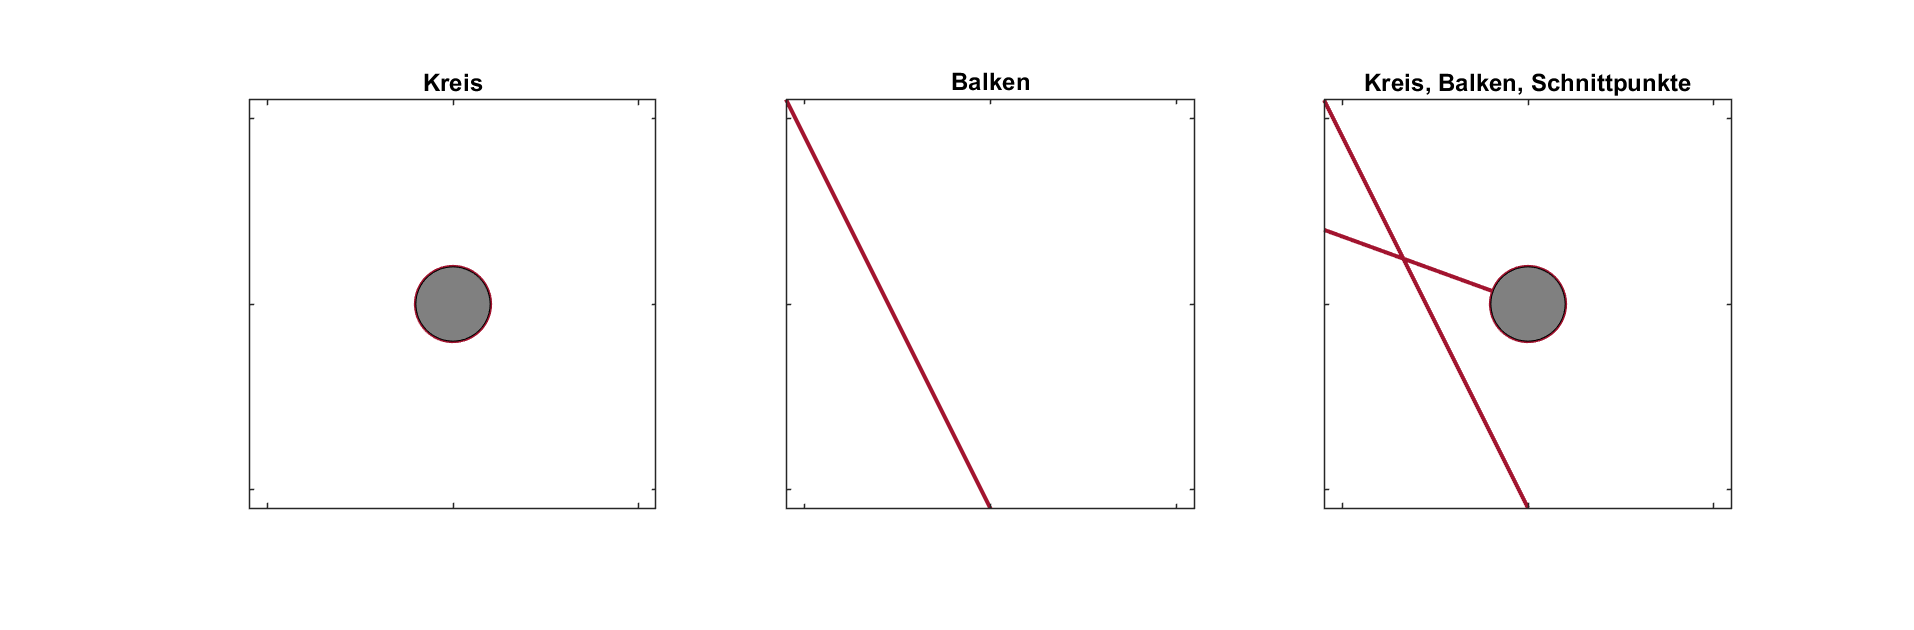
\includegraphics{img/Einheitskreis-Gestalt.png}
\caption{Components of a network. Created by ÉD.}
\end{figure}

    R is built in such a way that different libraries can be loaded for
different functions. For the network analysis we will use the package
\texttt{igraph}\footnote{https://igraph.org/r/}. With
\texttt{library(\textquotesingle{}igraph\textquotesingle{})} we load the
package.

With \texttt{if\ (!require("igraph"))\ install.packages("igraph")} we
install the package in case it is not available on the current system.

    \begin{tcolorbox}[breakable, size=fbox, boxrule=1pt, pad at break*=1mm,colback=cellbackground, colframe=cellborder]
\begin{Verbatim}[commandchars=\\\{\}]
\PY{n+nf}{if }\PY{p}{(}\PY{o}{!}\PY{n+nf}{require}\PY{p}{(}\PY{l+s}{\PYZdq{}}\PY{l+s}{igraph\PYZdq{}}\PY{p}{)}\PY{p}{)} \PY{n+nf}{install.packages}\PY{p}{(}\PY{l+s}{\PYZdq{}}\PY{l+s}{igraph\PYZdq{}}\PY{p}{)}
\PY{n+nf}{library}\PY{p}{(}\PY{l+s}{\PYZsq{}}\PY{l+s}{igraph\PYZsq{}}\PY{p}{)}
\end{Verbatim}
\end{tcolorbox}

    \hypertarget{the-dataset}{%
\subsection{The Dataset}\label{the-dataset}}

    The data basis is a two-column listing of the consortia. The first
column (\texttt{from}) contains the consortium whose \emph{letter of
intent} is evaluated. The second column (\texttt{to}) contains the
consortium which is named as cooperation partner.

This data is read in by means of the function \texttt{read.table}. There
are three parameters:

\begin{itemize}
\tightlist
\item
  \texttt{header=TRUE} (there is a header line in the dataset).
\item
  \texttt{sep=","} (the values are separated by a comma)
\item
  \texttt{text=""} (the values themselves are between the quotes)
\end{itemize}

We pass these values to the self-selected variable \texttt{NFDI\_edges}
, which is done with the arrow symbol pointing to the left.

The data itself comes from the GitHub gist
\href{https://gist.github.com/LukasCBossert/9bd04115db3aa9ed974fdc69d3ff227c}{nfdi-collaborations.csv}

    \begin{tcolorbox}[breakable, size=fbox, boxrule=1pt, pad at break*=1mm,colback=cellbackground, colframe=cellborder]
\begin{Verbatim}[commandchars=\\\{\}]
\PY{c+c1}{\PYZsh{} Dataset:}
\PY{c+c1}{\PYZsh{} https://gist.github.com/LukasCBossert/9bd04115db3aa9ed974fdc69d3ff227c}
\PY{n}{NFDI\PYZus{}edges} \PY{o}{\PYZlt{}\PYZhy{}} \PY{n+nf}{read.table}\PY{p}{(}\PY{n}{header}\PY{o}{=}\PY{k+kc}{TRUE}\PY{p}{,}
                         \PY{n}{sep}\PY{o}{=}\PY{l+s}{\PYZdq{}}\PY{l+s}{,\PYZdq{}}\PY{p}{,}
                         \PY{n}{text}\PY{o}{=}\PY{l+s}{\PYZdq{}}
\PY{l+s}{from,to}
\PY{l+s}{DataPLANT,NFDI4BioDiversity}
\PY{l+s}{DataPLANT,NFDI4Chem}
\PY{l+s}{GHGA,NFDI4Health}
\PY{l+s}{KonsortSWD,BERD@NFDI}
\PY{l+s}{KonsortSWD,NFDI4BioDiversity}
\PY{l+s}{KonsortSWD,NFDI4Earth}
\PY{l+s}{KonsortSWD,NFDI4Health}
\PY{l+s}{KonsortSWD,Text+}
\PY{l+s}{NFDI4BioDiversity,NFDI4Earth}
\PY{l+s}{NFDI4BioDiversity,NFDI4Chem}
\PY{l+s}{NFDI4BioDiversity,NFDI4Health}
\PY{l+s}{NFDI4BioDiversity,KonsortSWD}
\PY{l+s}{NFDI4BioDiversity,DataPLANT}
\PY{l+s}{NFDI4Cat,FAIRmat}
\PY{l+s}{NFDI4Cat,NFDI4Chem}
\PY{l+s}{NFDI4Cat,NFDI4Ing}
\PY{l+s}{NFDI4Cat,DAPHNE4NFDI}
\PY{l+s}{NFDI4Chem,FAIRmat}
\PY{l+s}{NFDI4Chem,NFDI4Ing}
\PY{l+s}{NFDI4Chem,NFDI4Cat}
\PY{l+s}{NFDI4Chem,DAPHNE4NFDI}
\PY{l+s}{NFDI4Chem,PUNCH}
\PY{l+s}{NFDI4Chem,NFDI4Health}
\PY{l+s}{NFDI4Chem,NFDI4BioDiversity}
\PY{l+s}{NFDI4Culture,Text+}
\PY{l+s}{NFDI4Culture,MaRDI}
\PY{l+s}{NFDI4Culture,NFDI4Ing}
\PY{l+s}{NFDI4Health,GHGA}
\PY{l+s}{NFDI4Health,KonsortSWD}
\PY{l+s}{NFDI4Health,NFDI4Chem}
\PY{l+s}{NFDI4Health,NFDI4Earth}
\PY{l+s}{NFDI4Health,NFDI4BioDiversity}
\PY{l+s}{NFDI4Ing,NFDI\PYZhy{}MatWerk}
\PY{l+s}{NFDI4Ing,FAIRmat}
\PY{l+s}{NFDI4Ing,NFDI4Chem}
\PY{l+s}{NFDI4Ing,NFDI4Earth}
\PY{l+s}{NFDI4Ing,MaRDI}
\PY{l+s}{NFDI4Ing,Text+}
\PY{l+s}{NFDI4Ing,NFDI4Culture}
\PY{l+s}{BERD@NFDI,KonsortSWD}
\PY{l+s}{BERD@NFDI,MaRDI}
\PY{l+s}{BERD@NFDI,Text+}
\PY{l+s}{DAPHNE4NFDI,FAIRmat}
\PY{l+s}{DAPHNE4NFDI,NFDI\PYZhy{}MatWerk}
\PY{l+s}{DAPHNE4NFDI,NFDI4Cat}
\PY{l+s}{DAPHNE4NFDI,NFDI4Chem}
\PY{l+s}{DAPHNE4NFDI,NFDI4Health}
\PY{l+s}{DAPHNE4NFDI,NFDI4Ing}
\PY{l+s}{DAPHNE4NFDI,PUNCH}
\PY{l+s}{FAIRmat,DAPHNE4NFDI}
\PY{l+s}{FAIRmat,DataPLANT}
\PY{l+s}{FAIRmat,MaRDI}
\PY{l+s}{FAIRmat,NFDI\PYZhy{}MatWerk}
\PY{l+s}{FAIRmat,NFDI4Cat}
\PY{l+s}{FAIRmat,NFDI4Chem}
\PY{l+s}{FAIRmat,DataScience}
\PY{l+s}{FAIRmat,NFDI4Ing}
\PY{l+s}{FAIRmat,PUNCH}
\PY{l+s}{MaRDI,BERD@NFDI}
\PY{l+s}{MaRDI,FAIRmat}
\PY{l+s}{MaRDI,NFDI\PYZhy{}MatWerk}
\PY{l+s}{MaRDI,NFDI4Cat}
\PY{l+s}{MaRDI,NFDI4Chem}
\PY{l+s}{MaRDI,NFDI4Ing}
\PY{l+s}{MaRDI,PUNCH}
\PY{l+s}{NFDI\PYZhy{}MatWerk,DAPHNE4NFDI}
\PY{l+s}{NFDI\PYZhy{}MatWerk,DataPLANT}
\PY{l+s}{NFDI\PYZhy{}MatWerk,FAIRmat}
\PY{l+s}{NFDI\PYZhy{}MatWerk,MaRDI}
\PY{l+s}{NFDI\PYZhy{}MatWerk,NFDI4Chem}
\PY{l+s}{NFDI\PYZhy{}MatWerk,DataScience}
\PY{l+s}{NFDI\PYZhy{}MatWerk,NFDI4Ing}
\PY{l+s}{DataScience,KonsortSWD}
\PY{l+s}{DataScience,MaRDI}
\PY{l+s}{DataScience,NFDI\PYZhy{}MatWerk}
\PY{l+s}{DataScience,NFDI4BioDiversity}
\PY{l+s}{DataScience,NFDI4Cat}
\PY{l+s}{DataScience,NFDI4Chem}
\PY{l+s}{DataScience,NFDI4Culture}
\PY{l+s}{DataScience,NFDI4Health}
\PY{l+s}{DataScience,NFDI4Ing}
\PY{l+s}{DataScience,NFDI4Microbiota}
\PY{l+s}{NFDI4Earth,DataPLANT}
\PY{l+s}{NFDI4Earth,GHGA}
\PY{l+s}{NFDI4Earth,KonsortSWD}
\PY{l+s}{NFDI4Earth,NFDI4BioDiversity}
\PY{l+s}{NFDI4Earth,NFDI4Cat}
\PY{l+s}{NFDI4Earth,NFDI4Chem}
\PY{l+s}{NFDI4Earth,NFDI4Culture}
\PY{l+s}{NFDI4Earth,NFDI4Health}
\PY{l+s}{NFDI4Earth,NFDI4Ing}
\PY{l+s}{NFDI4Microbiota,DataPLANT}
\PY{l+s}{NFDI4Microbiota,GHGA}
\PY{l+s}{NFDI4Microbiota,NFDI4BioDiversity}
\PY{l+s}{NFDI4Microbiota,NFDI4Chem}
\PY{l+s}{NFDI4Microbiota,DataScience}
\PY{l+s}{NFDI4Microbiota,NFDI4Health}
\PY{l+s}{NFDI4Microbiota,NFDI4Ing}
\PY{l+s}{PUNCH,DAPHNE4NFDI}
\PY{l+s}{PUNCH,FAIRmat}
\PY{l+s}{PUNCH,GHGA}
\PY{l+s}{PUNCH,MaRDI}
\PY{l+s}{PUNCH,NFDI4Earth}
\PY{l+s}{PUNCH,NFDI4Ing}
\PY{l+s}{Text+,KonsortSWD}
\PY{l+s}{Text+,NFDI4BioDiversity}
\PY{l+s}{Text+,NFDI4Culture}
\PY{l+s}{Text+,NFDI4Earth}
\PY{l+s}{Text+,NFDI4Ing}
\PY{l+s}{\PYZdq{}}\PY{p}{)}
\end{Verbatim}
\end{tcolorbox}

    So that we can create a network from this dataset, we have to prepare it
and create a \texttt{igraph\ graph}.\footnote{https://igraph.org/r/doc/graph\_from\_data\_frame.html}
This is done with the function \texttt{graph\_from\_data\_frame}, to
which we pass our dataset.

We also specify that our dataset or network is undirected
(\texttt{directed=FALSE}), that means that the direction as specified by
\texttt{from,to} in the dataset does not matter. All we care about now
is that two consortia are linked.

We pass this information to the variable \texttt{NFDI\_network}.

    \begin{tcolorbox}[breakable, size=fbox, boxrule=1pt, pad at break*=1mm,colback=cellbackground, colframe=cellborder]
\begin{Verbatim}[commandchars=\\\{\}]
\PY{n}{NFDI\PYZus{}network} \PY{o}{\PYZlt{}\PYZhy{}} \PY{n+nf}{graph\PYZus{}from\PYZus{}data\PYZus{}frame}\PY{p}{(}\PY{n}{NFDI\PYZus{}edges}\PY{p}{,}
                                      \PY{n}{directed} \PY{o}{=} \PY{k+kc}{FALSE}
                                     \PY{p}{)}
\end{Verbatim}
\end{tcolorbox}

    \hypertarget{basic-setting}{%
\subsection{Basic setting}\label{basic-setting}}

First, we will set a parameter so that our network always looks the same
when the data is the same. This parameter is \texttt{seed}. We choose an
arbitrary number, which may be large.

After that we come to the actual plot. For this we call the function
\texttt{plot} and pass it the variable of our network graph
\texttt{NFDI\_network}. For a title we can still specify the parameter
\texttt{main} and also we can specify if we want to have a frame around
the network with \texttt{frame=TRUE}.

    \begin{tcolorbox}[breakable, size=fbox, boxrule=1pt, pad at break*=1mm,colback=cellbackground, colframe=cellborder]
\begin{Verbatim}[commandchars=\\\{\}]
\PY{n+nf}{set.seed}\PY{p}{(}\PY{l+m}{9876543}\PY{p}{)}

\PY{n+nf}{plot}\PY{p}{(}\PY{n}{NFDI\PYZus{}network}\PY{p}{,}                    \PY{c+c1}{\PYZsh{} loading data frame}
     \PY{n}{main}  \PY{o}{=} \PY{l+s}{\PYZdq{}}\PY{l+s}{NFDI Network\PYZdq{}}\PY{p}{,}          \PY{c+c1}{\PYZsh{} adding a title}
     \PY{n}{frame} \PY{o}{=} \PY{k+kc}{TRUE}                     \PY{c+c1}{\PYZsh{} making a frame }
     \PY{p}{)}
\end{Verbatim}
\end{tcolorbox}

    \begin{center}
    \adjustimage{max size={0.9\linewidth}{0.9\paperheight}}{the-promise-to-partner_files/the-promise-to-partner_11_0.png}
    \end{center}
    { \hspace*{\fill} \\}
    
    We see the network of NFDI consortia without any other explicit
settings.

    \hypertarget{layout-settings}{%
\subsection{Layout settings}\label{layout-settings}}

The next step we want to do is optimize the layout of the network.
Instead of retyping the code for the plot, we will select the content of
the last cell, copy and paste it into the next cell.

We'll expand the code this way and work on the network step by step.

There are different algorithms for the layout of networks. Depending on
the data set, sometimes one layout, sometimes the other may be more
suitable. With the layout \texttt{graphopt}\footnote{https://igraph.org/r/doc/layout\_with\_graphopt.html}
you usually get a good result.

We pass this value \texttt{layout.graphopt} to the parameter
\texttt{layout}.

    \begin{tcolorbox}[breakable, size=fbox, boxrule=1pt, pad at break*=1mm,colback=cellbackground, colframe=cellborder]
\begin{Verbatim}[commandchars=\\\{\}]
\PY{n+nf}{set.seed}\PY{p}{(}\PY{l+m}{9876543}\PY{p}{)}

\PY{n+nf}{plot}\PY{p}{(}\PY{n}{NFDI\PYZus{}network}\PY{p}{,}                     \PY{c+c1}{\PYZsh{} loading data frame}
     \PY{n}{main}  \PY{o}{=} \PY{l+s}{\PYZdq{}}\PY{l+s}{NFDI Network\PYZdq{}}\PY{p}{,}           \PY{c+c1}{\PYZsh{} adding a title}
     \PY{n}{frame}  \PY{o}{=} \PY{k+kc}{TRUE}\PY{p}{,}                    \PY{c+c1}{\PYZsh{} making a frame}
     \PY{n}{layout} \PY{o}{=} \PY{n}{layout.graphopt}\PY{p}{,}         \PY{c+c1}{\PYZsh{}* better layout options}
     \PY{p}{)}
\end{Verbatim}
\end{tcolorbox}

    \begin{center}
    \adjustimage{max size={0.9\linewidth}{0.9\paperheight}}{the-promise-to-partner_files/the-promise-to-partner_14_0.png}
    \end{center}
    { \hspace*{\fill} \\}
    
    We see the network of NFDI consortia without any other explicit
settings.

    The network is now already better structured and the distances between
the nodes are more harmonious.

If you like, you can try out further layout settings \footnote{https://igraph.org/python/doc/tutorial/tutorial.html\#layout-algorithms}:

\begin{itemize}
\tightlist
\item
  \texttt{layout\_circle} (\texttt{circle,circular}): Deterministic
  layout that places the vertices on a circle
\item
  \texttt{layout\_drl} (\texttt{drl}): The Distributed Recursive Layout
  algorithm for large graphs
\item
  \texttt{layout\_fruchterman\_reingold} (\texttt{fr}):
  Fruchterman-Reingold force-directed algorithm
\item
  \texttt{layout\_fruchterman\_reingold\_3d} (\texttt{fr3d,\ fr\_3d}):
  Fruchterman-Reingold force-directed algorithm in three dimensions
\item
  \texttt{layout\_grid\_fruchterman\_reingold} (\texttt{grid\_fr}):
  Fruchterman-Reingold force-directed algorithm with grid heuristics for
  large graphs
\item
  \texttt{layout\_kamada\_kawai} (\texttt{kk}): Kamada-Kawai
  force-directed algorithm
\item
  \texttt{layout\_kamada\_kawai\_3d} (\texttt{kk3d,\ kk\_3d}):
  Kamada-Kawai force-directed algorithm in three dimensions
\item
  \texttt{layout\_lgl} (\texttt{large,\ lgl,\ large\_graph}): The Large
  Graph Layout algorithm for large graphs
\item
  \texttt{layout\_random} (\texttt{random}): Places the vertices
  completely randomly
\item
  \texttt{layout\_random\_3d} (\texttt{random\_3d}): Places the vertices
  completely randomly in 3D
\item
  \texttt{layout\_reingold\_tilford} (\texttt{rt,\ tree}):
  Reingold-Tilford tree layout, useful for (almost) tree-like graphs
\item
  \texttt{layout\_reingold\_tilford\_circular}
  (\texttt{rt\_circular,\ tree}): Reingold-Tilford tree layout with a
  polar coordinate post-transformation, useful for (almost) tree-like
  graphs
\item
  \texttt{layout\_sphere} (\texttt{sphere,spherical,circular\_3d}):
  Deterministic layout that places the vertices evenly on the surface of
  a sphere
\end{itemize}

    \hypertarget{color-size-curvature-nodes-and-edges}{%
\subsubsection{Color, Size, Curvature (Nodes and
Edges)}\label{color-size-curvature-nodes-and-edges}}

After we have optimized the arrangement of the nodes, let's tackle the
representation of the nodes and edges in the next step.

Various parameters can be adjusted according to your own wishes.

First we want to tackle the color of the nodes. The parameter is
\texttt{vertex.color} and we can specify an HTML color value (for
example \texttt{\#ffcc66}).\footnote{https://www.w3schools.com/colors/colors\_picker.asp}
For the border of the nodes we choose the same color code. The parameter
is \texttt{vertex.frame.color}.

The labels of the nodes can also be modified. The change of the font
size is done by the parameter \texttt{vertex.label.cex}, to which we
pass the value \texttt{0.5}. It is important here that the value is
\emph{not} written in quotes. This is a relative size and we want the
labels to be half the size they were in the previous network. The color
of the label can also be changed. Quite analogously, the parameter is
called \texttt{vertex.label.color}, to which we can also pass the color
value as a string, such as \texttt{"black"}.

A network consists not only of nodes but also of edges connecting two
nodes. For the color change we need the parameter \texttt{edge.color},
to which we pass for example \texttt{"\#808080"}. Besides the color we
can also specify the degree of ``curvature'', which is set with
\texttt{edge.curved} and the value \texttt{0.1}. Again, it is important
that \emph{no} quotes are set.

    \begin{tcolorbox}[breakable, size=fbox, boxrule=1pt, pad at break*=1mm,colback=cellbackground, colframe=cellborder]
\begin{Verbatim}[commandchars=\\\{\}]
\PY{n+nf}{set.seed}\PY{p}{(}\PY{l+m}{9876543}\PY{p}{)}


\PY{n+nf}{plot}\PY{p}{(}\PY{n}{NFDI\PYZus{}network}\PY{p}{,}                     \PY{c+c1}{\PYZsh{} loading data frame}
     \PY{n}{main}   \PY{o}{=} \PY{l+s}{\PYZdq{}}\PY{l+s}{NFDI Network\PYZdq{}}\PY{p}{,}          \PY{c+c1}{\PYZsh{} adding a title}
     \PY{n}{frame}  \PY{o}{=} \PY{k+kc}{TRUE}\PY{p}{,}                    \PY{c+c1}{\PYZsh{} making a frame }
     \PY{n}{layout} \PY{o}{=} \PY{n}{layout.graphopt}\PY{p}{,}         \PY{c+c1}{\PYZsh{} better layout options}
     \PY{n}{vertex.color}       \PY{o}{=} \PY{l+s}{\PYZdq{}}\PY{l+s}{\PYZsh{}ffcc66\PYZdq{}}\PY{p}{,}   \PY{c+c1}{\PYZsh{}* color of nodes}
     \PY{n}{vertex.frame.color} \PY{o}{=} \PY{l+s}{\PYZdq{}}\PY{l+s}{\PYZsh{}ffcc66\PYZdq{}}\PY{p}{,}   \PY{c+c1}{\PYZsh{}* color of the frame of nodes}
     \PY{n}{vertex.label.cex}   \PY{o}{=} \PY{l+m}{0.5}\PY{p}{,}         \PY{c+c1}{\PYZsh{}* size of the description of the labels}
     \PY{n}{vertex.label.color} \PY{o}{=} \PY{l+s}{\PYZdq{}}\PY{l+s}{black\PYZdq{}}\PY{p}{,}     \PY{c+c1}{\PYZsh{}* color of the description }
     \PY{n}{edge.color}         \PY{o}{=} \PY{l+s}{\PYZdq{}}\PY{l+s}{\PYZsh{}808080\PYZdq{}}\PY{p}{,}   \PY{c+c1}{\PYZsh{}* color of edges}
     \PY{n}{edge.curved}        \PY{o}{=} \PY{l+m}{0.1}\PY{p}{,}         \PY{c+c1}{\PYZsh{}* factor of \PYZdq{}curvity\PYZdq{}}
     \PY{p}{)}
\end{Verbatim}
\end{tcolorbox}

    \begin{center}
    \adjustimage{max size={0.9\linewidth}{0.9\paperheight}}{the-promise-to-partner_files/the-promise-to-partner_18_0.png}
    \end{center}
    { \hspace*{\fill} \\}
    
    \hypertarget{node-size-as-a-function-of-the-number-of-edges}{%
\subsection{Node size as a function of the number of
edges}\label{node-size-as-a-function-of-the-number-of-edges}}

In the previous network representations, all nodes are the same size.

Now we want to add another layer of information and output the node size
according to the number of its edges.

We can determine the number of edges per node with the function
\texttt{degree}\footnote{https://igraph.org/r/doc/degree.html}. If we
pass this function the dataset of the network
(\texttt{degree(NFDI\_network)}), then we get the number of edges per
node. We take these values as the size specification for the nodes.

We thus extend the previous code by one line. The node size is hidden
behind the parameter \texttt{vertex.size} and as value we pass the
function \texttt{degree(NFDI\_network)}.

    \begin{tcolorbox}[breakable, size=fbox, boxrule=1pt, pad at break*=1mm,colback=cellbackground, colframe=cellborder]
\begin{Verbatim}[commandchars=\\\{\}]
\PY{c+c1}{\PYZsh{}data.frame(}
    \PY{n+nf}{degree}\PY{p}{(}\PY{n}{NFDI\PYZus{}network}\PY{p}{)} \PY{c+c1}{\PYZsh{}* calculate number of edges}
\PY{c+c1}{\PYZsh{})}
\end{Verbatim}
\end{tcolorbox}

    \begin{description*}
\item[DataPLANT] 7
\item[GHGA] 5
\item[KonsortSWD] 11
\item[NFDI4BioDiversity] 13
\item[NFDI4Cat] 10
\item[NFDI4Chem] 19
\item[NFDI4Culture] 7
\item[NFDI4Health] 13
\item[NFDI4Ing] 19
\item[BERD@NFDI] 5
\item[DAPHNE4NFDI] 12
\item[FAIRmat] 16
\item[MaRDI] 14
\item[NFDI-MatWerk] 12
\item[DataScience] 13
\item[NFDI4Earth] 15
\item[NFDI4Microbiota] 8
\item[PUNCH] 10
\item[Text+] 9
\end{description*}


    
    \begin{tcolorbox}[breakable, size=fbox, boxrule=1pt, pad at break*=1mm,colback=cellbackground, colframe=cellborder]
\begin{Verbatim}[commandchars=\\\{\}]
\PY{n+nf}{set.seed}\PY{p}{(}\PY{l+m}{9876543}\PY{p}{)}

\PY{n+nf}{plot}\PY{p}{(}\PY{n}{NFDI\PYZus{}network}\PY{p}{,}                     \PY{c+c1}{\PYZsh{} loading data frame}
     \PY{n}{main}   \PY{o}{=} \PY{l+s}{\PYZdq{}}\PY{l+s}{NFDI\PYZhy{}Netzwerk\PYZdq{}}\PY{p}{,}         \PY{c+c1}{\PYZsh{} adding a title}
     \PY{n}{frame}  \PY{o}{=} \PY{k+kc}{TRUE}\PY{p}{,}                    \PY{c+c1}{\PYZsh{} making a frame }
     \PY{n}{layout} \PY{o}{=} \PY{n}{layout.graphopt}\PY{p}{,}         \PY{c+c1}{\PYZsh{} better layout options}
     \PY{n}{vertex.color}       \PY{o}{=} \PY{l+s}{\PYZdq{}}\PY{l+s}{\PYZsh{}ffcc66\PYZdq{}}\PY{p}{,}   \PY{c+c1}{\PYZsh{} color of nodes}
     \PY{n}{vertex.frame.color} \PY{o}{=} \PY{l+s}{\PYZdq{}}\PY{l+s}{\PYZsh{}ffcc66\PYZdq{}}\PY{p}{,}   \PY{c+c1}{\PYZsh{} color of the frame of nodes}
     \PY{n}{vertex.label.cex}   \PY{o}{=} \PY{l+m}{0.5}\PY{p}{,}         \PY{c+c1}{\PYZsh{} size of the description of the labels}
     \PY{n}{vertex.label.color} \PY{o}{=} \PY{l+s}{\PYZdq{}}\PY{l+s}{black\PYZdq{}}\PY{p}{,}     \PY{c+c1}{\PYZsh{} color of the description }
                                       \PY{c+c1}{\PYZsh{} color: https://www.w3schools.com/colors/colors\PYZus{}picker.asp }
     \PY{n}{edge.color}         \PY{o}{=} \PY{l+s}{\PYZdq{}}\PY{l+s}{\PYZsh{}808080\PYZdq{}}\PY{p}{,}   \PY{c+c1}{\PYZsh{} color of edges}
     \PY{n}{edge.curved}        \PY{o}{=} \PY{l+m}{0.1}\PY{p}{,}         \PY{c+c1}{\PYZsh{} factor of \PYZdq{}curvity\PYZdq{}}
     \PY{n}{vertex.size}        \PY{o}{=} \PY{n+nf}{degree}\PY{p}{(}\PY{n}{NFDI\PYZus{}network}\PY{p}{)}\PY{p}{,} \PY{c+c1}{\PYZsh{}* size of nodes depends on amount of edges}
     \PY{p}{)}
\end{Verbatim}
\end{tcolorbox}

    \begin{center}
    \adjustimage{max size={0.9\linewidth}{0.9\paperheight}}{the-promise-to-partner_files/the-promise-to-partner_21_0.png}
    \end{center}
    { \hspace*{\fill} \\}
    
    \hypertarget{node-size-as-a-function-of-the-number-of-incoming-and-outgoing-edges.}{%
\subsection{Node size as a function of the number of incoming and
outgoing
edges.}\label{node-size-as-a-function-of-the-number-of-incoming-and-outgoing-edges.}}

We have now introduced a second layer of information into our network
and can display the node size in relation to the number of edges.

In the next step, we would like to introduce another component. Until
now, it was irrelevant whether a consortium was named first or second in
the dataset, i.e., it was irrelevant whether it was the active or the
passive collaborator.

Now we would like to consider the distinction in the network. To do
this, our graph (network) must be ``directed''\footnote{https://en.wikipedia.org/wiki/Directed\_graph}.

We introduce a new variable (\texttt{NFDI\_network\_directed}), which
contains the dataset as a directed graph, which we set with
\texttt{directed\ =\ TRUE}.

    \begin{tcolorbox}[breakable, size=fbox, boxrule=1pt, pad at break*=1mm,colback=cellbackground, colframe=cellborder]
\begin{Verbatim}[commandchars=\\\{\}]
\PY{n}{NFDI\PYZus{}network\PYZus{}directed} \PY{o}{\PYZlt{}\PYZhy{}} \PY{n+nf}{graph\PYZus{}from\PYZus{}data\PYZus{}frame}\PY{p}{(}\PY{n}{NFDI\PYZus{}edges}\PY{p}{,}
                                               \PY{n}{directed} \PY{o}{=} \PY{k+kc}{TRUE}
                                              \PY{p}{)}
\end{Verbatim}
\end{tcolorbox}

    We transfer the remaining plot data from the previous cell. It is now
crucial that we pass the new variable with the directed graph to the
plot function. In addition, we also pass the new variable to the
\texttt{degree} function.

In the directed network, the curvature of the edges makes it difficult
to read. Therefore we choose the value \texttt{0} for
\texttt{edge.curved}.

Likewise, the arrowheads should become smaller, which is possible with
\texttt{edge.arrow.size} and the relative value \texttt{0.5}.

    \begin{tcolorbox}[breakable, size=fbox, boxrule=1pt, pad at break*=1mm,colback=cellbackground, colframe=cellborder]
\begin{Verbatim}[commandchars=\\\{\}]
\PY{n+nf}{set.seed}\PY{p}{(}\PY{l+m}{9876543}\PY{p}{)}

\PY{n+nf}{plot}\PY{p}{(}\PY{n}{NFDI\PYZus{}network\PYZus{}directed}\PY{p}{,}            \PY{c+c1}{\PYZsh{}\PYZlt{}\PYZlt{}\PYZlt{}\PYZlt{}\PYZlt{}\PYZlt{}\PYZlt{} loading data frame}
     \PY{n}{main}   \PY{o}{=} \PY{l+s}{\PYZdq{}}\PY{l+s}{NFDI\PYZhy{}Netzwerk\PYZdq{}}\PY{p}{,}         \PY{c+c1}{\PYZsh{} adding a title}
     \PY{n}{frame}  \PY{o}{=} \PY{k+kc}{TRUE}\PY{p}{,}                    \PY{c+c1}{\PYZsh{} making a frame }
     \PY{n}{layout} \PY{o}{=} \PY{n}{layout.graphopt}\PY{p}{,}         \PY{c+c1}{\PYZsh{} better layout options}
     \PY{n}{vertex.color}       \PY{o}{=} \PY{l+s}{\PYZdq{}}\PY{l+s}{\PYZsh{}ffcc66\PYZdq{}}\PY{p}{,}   \PY{c+c1}{\PYZsh{} color of nodes}
     \PY{n}{vertex.frame.color} \PY{o}{=} \PY{l+s}{\PYZdq{}}\PY{l+s}{\PYZsh{}ffcc66\PYZdq{}}\PY{p}{,}   \PY{c+c1}{\PYZsh{} color of the frame of nodes}
     \PY{n}{vertex.label.cex}   \PY{o}{=} \PY{l+m}{0.5}\PY{p}{,}         \PY{c+c1}{\PYZsh{} size of the description of the labels}
     \PY{n}{vertex.label.color} \PY{o}{=} \PY{l+s}{\PYZdq{}}\PY{l+s}{black\PYZdq{}}\PY{p}{,}     \PY{c+c1}{\PYZsh{} color of the description }
                                       \PY{c+c1}{\PYZsh{} color: https://www.w3schools.com/colors/colors\PYZus{}picker.asp }
     \PY{n}{edge.color}         \PY{o}{=} \PY{l+s}{\PYZdq{}}\PY{l+s}{\PYZsh{}808080\PYZdq{}}\PY{p}{,}   \PY{c+c1}{\PYZsh{} color of edges}
     \PY{n}{edge.curved}        \PY{o}{=} \PY{l+m}{0}\PY{p}{,}           \PY{c+c1}{\PYZsh{}\PYZlt{}\PYZlt{}\PYZlt{}\PYZlt{}\PYZlt{}\PYZlt{}\PYZlt{}\PYZlt{}\PYZlt{} factor of \PYZdq{}curvity\PYZdq{}}
     \PY{n}{vertex.size}        \PY{o}{=} \PY{n+nf}{degree}\PY{p}{(}\PY{n}{NFDI\PYZus{}network\PYZus{}directed}\PY{p}{)}\PY{p}{,} \PY{c+c1}{\PYZsh{}\PYZlt{}\PYZlt{}\PYZlt{}\PYZlt{}\PYZlt{}\PYZlt{} size of nodes depends on amount of edges}
     \PY{n}{edge.arrow.size}    \PY{o}{=} \PY{n}{.}\PY{l+m}{5}\PY{p}{,}          \PY{c+c1}{\PYZsh{}* arrow size,  defaults to 1}
    \PY{p}{)}
\end{Verbatim}
\end{tcolorbox}

    \begin{center}
    \adjustimage{max size={0.9\linewidth}{0.9\paperheight}}{the-promise-to-partner_files/the-promise-to-partner_25_0.png}
    \end{center}
    { \hspace*{\fill} \\}
    
    In the next step, we want to scale the node size according to the
\emph{in}bound edges. The more often a consortium is named as a
collaborator, the larger its node will be.

We can modify the function \texttt{degree} for this by adding
\texttt{mode\ =\ "in"}\footnote{https://igraph.org/r/doc/degree.html}.

\begin{Shaded}
\begin{Highlighting}[]
\NormalTok{degree(NFDI\_network\_directed,}
\NormalTok{       mode = "in")}
\end{Highlighting}
\end{Shaded}

    \begin{tcolorbox}[breakable, size=fbox, boxrule=1pt, pad at break*=1mm,colback=cellbackground, colframe=cellborder]
\begin{Verbatim}[commandchars=\\\{\}]
\PY{c+c1}{\PYZsh{}data.frame(}
    \PY{n+nf}{degree}\PY{p}{(}\PY{n}{NFDI\PYZus{}network\PYZus{}directed}\PY{p}{,}
                  \PY{n}{mode} \PY{o}{=} \PY{l+s}{\PYZdq{}}\PY{l+s}{in\PYZdq{}}\PY{p}{)}
\PY{c+c1}{\PYZsh{})}
\end{Verbatim}
\end{tcolorbox}

    \begin{description*}
\item[DataPLANT] 5
\item[GHGA] 4
\item[KonsortSWD] 6
\item[NFDI4BioDiversity] 8
\item[NFDI4Cat] 6
\item[NFDI4Chem] 12
\item[NFDI4Culture] 4
\item[NFDI4Health] 8
\item[NFDI4Ing] 12
\item[BERD@NFDI] 2
\item[DAPHNE4NFDI] 5
\item[FAIRmat] 7
\item[MaRDI] 7
\item[NFDI-MatWerk] 5
\item[DataScience] 3
\item[NFDI4Earth] 6
\item[NFDI4Microbiota] 1
\item[PUNCH] 4
\item[Text+] 4
\end{description*}


    
    \begin{tcolorbox}[breakable, size=fbox, boxrule=1pt, pad at break*=1mm,colback=cellbackground, colframe=cellborder]
\begin{Verbatim}[commandchars=\\\{\}]
\PY{n+nf}{set.seed}\PY{p}{(}\PY{l+m}{9876543}\PY{p}{)}

\PY{n+nf}{plot}\PY{p}{(}\PY{n}{NFDI\PYZus{}network\PYZus{}directed}\PY{p}{,}            \PY{c+c1}{\PYZsh{} loading data frame}
     \PY{n}{main}   \PY{o}{=} \PY{l+s}{\PYZdq{}}\PY{l+s}{NFDI Network (\PYZlt{}in\PYZgt{})\PYZdq{}}\PY{p}{,}  \PY{c+c1}{\PYZsh{}\PYZlt{}\PYZlt{}\PYZlt{}\PYZlt{}\PYZlt{}\PYZlt{}\PYZlt{}\PYZlt{} adding a title}
     \PY{n}{frame}  \PY{o}{=} \PY{k+kc}{TRUE}\PY{p}{,}                    \PY{c+c1}{\PYZsh{} making a frame }
     \PY{n}{layout} \PY{o}{=} \PY{n}{layout.graphopt}\PY{p}{,}         \PY{c+c1}{\PYZsh{} better layout options}
     \PY{n}{vertex.color}       \PY{o}{=} \PY{l+s}{\PYZdq{}}\PY{l+s}{\PYZsh{}ffcc66\PYZdq{}}\PY{p}{,}   \PY{c+c1}{\PYZsh{} color of nodes}
     \PY{n}{vertex.frame.color} \PY{o}{=} \PY{l+s}{\PYZdq{}}\PY{l+s}{\PYZsh{}ffcc66\PYZdq{}}\PY{p}{,}   \PY{c+c1}{\PYZsh{} color of the frame of nodes}
     \PY{n}{vertex.label.cex}   \PY{o}{=} \PY{l+m}{0.5}\PY{p}{,}         \PY{c+c1}{\PYZsh{} size of the description of the labels}
     \PY{n}{vertex.label.color} \PY{o}{=} \PY{l+s}{\PYZdq{}}\PY{l+s}{black\PYZdq{}}\PY{p}{,}     \PY{c+c1}{\PYZsh{} color of the description }
                                       \PY{c+c1}{\PYZsh{} color: https://www.w3schools.com/colors/colors\PYZus{}picker.asp }
     \PY{n}{edge.color}         \PY{o}{=} \PY{l+s}{\PYZdq{}}\PY{l+s}{\PYZsh{}808080\PYZdq{}}\PY{p}{,}   \PY{c+c1}{\PYZsh{} color of edges}
     \PY{n}{edge.curved}        \PY{o}{=} \PY{l+m}{0}\PY{p}{,}           \PY{c+c1}{\PYZsh{} factor of \PYZdq{}curvity\PYZdq{}}
     \PY{n}{vertex.size}        \PY{o}{=} \PY{n+nf}{degree}\PY{p}{(}\PY{n}{NFDI\PYZus{}network\PYZus{}directed}\PY{p}{,}
                                 \PY{n}{mode} \PY{o}{=} \PY{l+s}{\PYZdq{}}\PY{l+s}{in\PYZdq{}}\PY{p}{)}\PY{p}{,} \PY{c+c1}{\PYZsh{}\PYZlt{}\PYZlt{}\PYZlt{}\PYZlt{}\PYZlt{}\PYZlt{} size of nodes depends on amount of edges}
     \PY{n}{edge.arrow.size}    \PY{o}{=} \PY{n}{.}\PY{l+m}{5}\PY{p}{,}          \PY{c+c1}{\PYZsh{} arrow size,  defaults to 1}
    \PY{p}{)}
\end{Verbatim}
\end{tcolorbox}

    \begin{center}
    \adjustimage{max size={0.9\linewidth}{0.9\paperheight}}{the-promise-to-partner_files/the-promise-to-partner_28_0.png}
    \end{center}
    { \hspace*{\fill} \\}
    
    Likewise, we can now also display the size of the consortia according to
their \emph{out}going edges.

We take the complete cell content from before and only change
\texttt{in} to \texttt{out}.

    \begin{tcolorbox}[breakable, size=fbox, boxrule=1pt, pad at break*=1mm,colback=cellbackground, colframe=cellborder]
\begin{Verbatim}[commandchars=\\\{\}]
\PY{c+c1}{\PYZsh{}data.frame(}
    \PY{n+nf}{degree}\PY{p}{(}\PY{n}{NFDI\PYZus{}network\PYZus{}directed}\PY{p}{,}
                  \PY{n}{mode} \PY{o}{=} \PY{l+s}{\PYZdq{}}\PY{l+s}{out\PYZdq{}}\PY{p}{)}
\PY{c+c1}{\PYZsh{})}
\end{Verbatim}
\end{tcolorbox}

    \begin{description*}
\item[DataPLANT] 2
\item[GHGA] 1
\item[KonsortSWD] 5
\item[NFDI4BioDiversity] 5
\item[NFDI4Cat] 4
\item[NFDI4Chem] 7
\item[NFDI4Culture] 3
\item[NFDI4Health] 5
\item[NFDI4Ing] 7
\item[BERD@NFDI] 3
\item[DAPHNE4NFDI] 7
\item[FAIRmat] 9
\item[MaRDI] 7
\item[NFDI-MatWerk] 7
\item[DataScience] 10
\item[NFDI4Earth] 9
\item[NFDI4Microbiota] 7
\item[PUNCH] 6
\item[Text+] 5
\end{description*}


    
    \begin{tcolorbox}[breakable, size=fbox, boxrule=1pt, pad at break*=1mm,colback=cellbackground, colframe=cellborder]
\begin{Verbatim}[commandchars=\\\{\}]
\PY{n+nf}{set.seed}\PY{p}{(}\PY{l+m}{9876543}\PY{p}{)}

\PY{n+nf}{plot}\PY{p}{(}\PY{n}{NFDI\PYZus{}network\PYZus{}directed}\PY{p}{,}            \PY{c+c1}{\PYZsh{} loading data frame}
     \PY{n}{main}   \PY{o}{=} \PY{l+s}{\PYZdq{}}\PY{l+s}{NFDI Network (\PYZlt{}out\PYZgt{})\PYZdq{}}\PY{p}{,}  \PY{c+c1}{\PYZsh{}\PYZlt{}\PYZlt{}\PYZlt{}\PYZlt{}\PYZlt{}\PYZlt{}\PYZlt{}\PYZlt{} adding a title}
     \PY{n}{frame}  \PY{o}{=} \PY{k+kc}{TRUE}\PY{p}{,}                    \PY{c+c1}{\PYZsh{} making a frame }
     \PY{n}{layout} \PY{o}{=} \PY{n}{layout.graphopt}\PY{p}{,}         \PY{c+c1}{\PYZsh{} better layout options}
     \PY{n}{vertex.color}       \PY{o}{=} \PY{l+s}{\PYZdq{}}\PY{l+s}{\PYZsh{}ffcc66\PYZdq{}}\PY{p}{,}   \PY{c+c1}{\PYZsh{} color of nodes}
     \PY{n}{vertex.frame.color} \PY{o}{=} \PY{l+s}{\PYZdq{}}\PY{l+s}{\PYZsh{}ffcc66\PYZdq{}}\PY{p}{,}   \PY{c+c1}{\PYZsh{} color of the frame of nodes}
     \PY{n}{vertex.label.cex}   \PY{o}{=} \PY{l+m}{0.5}\PY{p}{,}         \PY{c+c1}{\PYZsh{} size of the description of the labels}
     \PY{n}{vertex.label.color} \PY{o}{=} \PY{l+s}{\PYZdq{}}\PY{l+s}{black\PYZdq{}}\PY{p}{,}     \PY{c+c1}{\PYZsh{} color of the description }
                                       \PY{c+c1}{\PYZsh{} color: https://www.w3schools.com/colors/colors\PYZus{}picker.asp }
     \PY{n}{edge.color}         \PY{o}{=} \PY{l+s}{\PYZdq{}}\PY{l+s}{\PYZsh{}808080\PYZdq{}}\PY{p}{,}   \PY{c+c1}{\PYZsh{} color of edges}
     \PY{n}{edge.curved}        \PY{o}{=} \PY{l+m}{0}\PY{p}{,}           \PY{c+c1}{\PYZsh{} factor of \PYZdq{}curvity\PYZdq{}}
     \PY{n}{vertex.size}        \PY{o}{=} \PY{n+nf}{degree}\PY{p}{(}\PY{n}{NFDI\PYZus{}network\PYZus{}directed}\PY{p}{,}
                                 \PY{n}{mode} \PY{o}{=} \PY{l+s}{\PYZdq{}}\PY{l+s}{out\PYZdq{}}\PY{p}{)}\PY{p}{,} \PY{c+c1}{\PYZsh{}\PYZlt{}\PYZlt{}\PYZlt{}\PYZlt{}\PYZlt{}\PYZlt{} size of nodes depends on amount of edges}
     \PY{n}{edge.arrow.size}    \PY{o}{=} \PY{n}{.}\PY{l+m}{5}\PY{p}{,}          \PY{c+c1}{\PYZsh{} arrow size,  defaults to 1}
    \PY{p}{)}
\end{Verbatim}
\end{tcolorbox}

    \begin{center}
    \adjustimage{max size={0.9\linewidth}{0.9\paperheight}}{the-promise-to-partner_files/the-promise-to-partner_31_0.png}
    \end{center}
    { \hspace*{\fill} \\}
    
    It is noticeable that some nodes are shrinking and in the table you can
see that they have the value \texttt{0} for outgoing edges. This is
because these are the consortia that were already approved in the first
funding round and therefore did not submit a new Letter of Intent. After
all, our dataset only considers the Letters of Intent from the second
funding round. The consortia of the first round can therefore only be
mentioned as ``passive'' cooperation partners.

    \hypertarget{network-analysis}{%
\section{Network analysis}\label{network-analysis}}

After the previous rounds of network visualization, let's go one step
further and analyze the network structure.

\hypertarget{nfdi-conference-systematics}{%
\subsection{NFDI conference
systematics}\label{nfdi-conference-systematics}}

As a first step, let's color the nodes or consortia in the colors of the
NFDI conference systematics.

How does the NFDI conference systematics come about? Five panels have
been set up for the presentations:

\begin{enumerate}
\def\labelenumi{\arabic{enumi}.}
\tightlist
\item
  Medicine
\item
  Life Sciences
\item
  Humanities
\item
  Engineering Sciences
\item
  Chemistry/Physics
\end{enumerate}

    The applicant consortia were divided among these five groups:\footnote{https://www.dfg.de/download/pdf/foerderung/programme/nfdi/nfdi\_konferenz\_2020/programm\_webkonferenz\_2020.pdf}

\begin{figure}
\centering
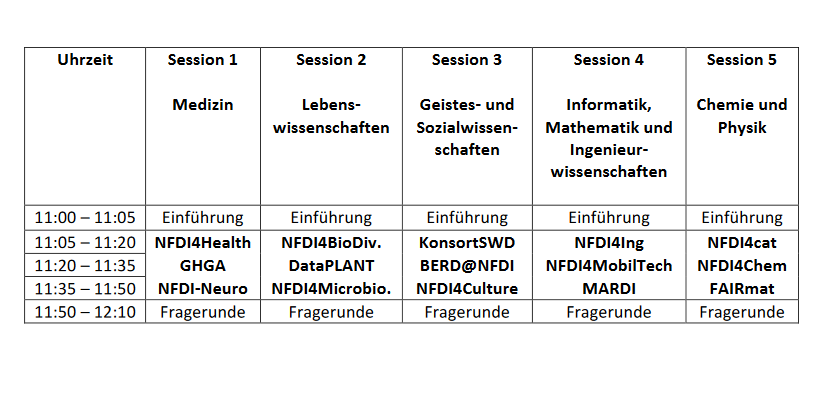
\includegraphics{img/nfdi-konferenzsystematik.png}
\caption{NFDI conference systematics}
\end{figure}

In the following, we abbreviate Group 4 ``Computer Science, Mathematics
and Engineering'' as ``Engineering''.

    It is noticeable that according to the DFG subject classification
system, the natural sciences have been divided between the life
sciences, engineering sciences and chemistry/physics, as can be seen in
the following Sankey (flow chart).

\begin{figure}
\centering
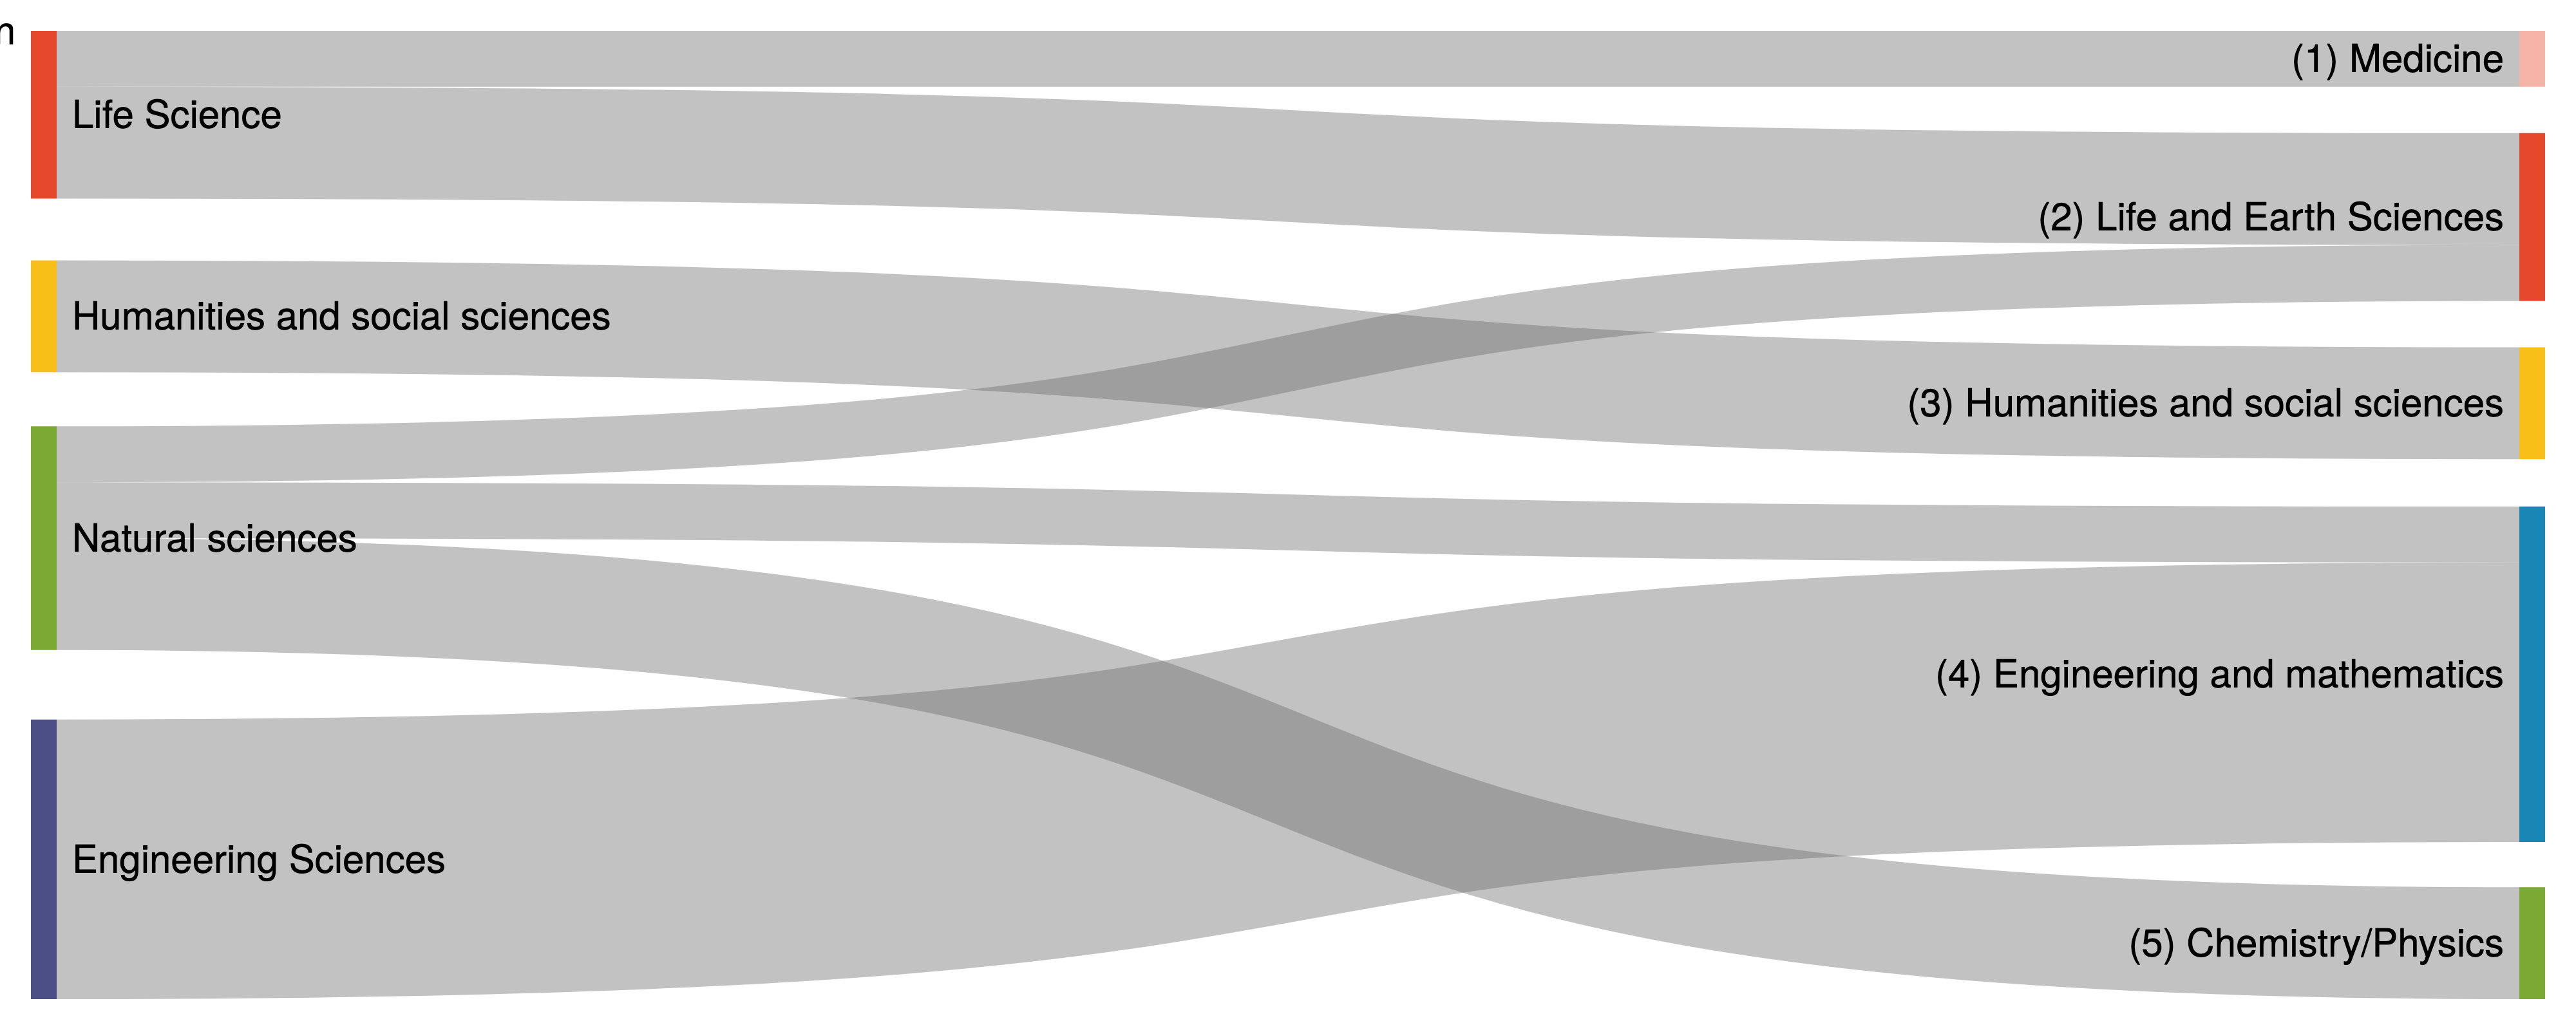
\includegraphics{img/dfg-nfdi-sankey.png}
\caption{Sankey diagram showing the change in subject affiliation
between DFG subject classification and NFDI conference classification.}
\end{figure}

So all consortia have been assigned to one of these five areas and we
now want to show this in the network. We load this classification of the
consortia on the conference system in the next cell.

This new record is passed to the variable `NFDI\_nodes'; the first
column contains the consortium names, the second column the number from
the NFDI-\emph{conference}systematics. The third column contains the
round in which the consortium was approved: \texttt{1}= 2019,
\texttt{2}= 2020.

The data can be read from the public GitHub gist
\href{https://gist.github.com/LukasCBossert/ce56ebd0059b4879c7d11c1090118c25}{nfdi-consortia.csv}.

    \begin{tcolorbox}[breakable, size=fbox, boxrule=1pt, pad at break*=1mm,colback=cellbackground, colframe=cellborder]
\begin{Verbatim}[commandchars=\\\{\}]
\PY{c+c1}{\PYZsh{} Dataset}
\PY{c+c1}{\PYZsh{} https://gist.github.com/LukasCBossert/ce56ebd0059b4879c7d11c1090118c25}
\PY{n}{NFDI\PYZus{}nodes} \PY{o}{\PYZlt{}\PYZhy{}} \PY{n+nf}{read.table}\PY{p}{(}\PY{n}{header}\PY{o}{=}\PY{k+kc}{TRUE}\PY{p}{,}
                         \PY{n}{sep}\PY{o}{=}\PY{l+s}{\PYZdq{}}\PY{l+s}{,\PYZdq{}}\PY{p}{,}
                         \PY{n}{text}\PY{o}{=}\PY{l+s}{\PYZdq{}}
\PY{l+s}{name,group,round}
\PY{l+s}{DataPLANT,2,1}
\PY{l+s}{GHGA,1,1}
\PY{l+s}{KonsortSWD,3,1}
\PY{l+s}{NFDI4BioDiversity,2,1}
\PY{l+s}{NFDI4Cat,5,1}
\PY{l+s}{NFDI4Chem,5,1}
\PY{l+s}{NFDI4Culture,3,1}
\PY{l+s}{NFDI4Health,1,1}
\PY{l+s}{NFDI4Ing,4,1}
\PY{l+s}{BERD@NFDI,3,2}
\PY{l+s}{DAPHNE4NFDI,5,2}
\PY{l+s}{FAIRmat,5,2}
\PY{l+s}{MaRDI,4,2}
\PY{l+s}{NFDI\PYZhy{}MatWerk,4,2}
\PY{l+s}{DataScience,4,2}
\PY{l+s}{NFDI4Earth,2,2}
\PY{l+s}{NFDI4Microbiota,2,2}
\PY{l+s}{PUNCH,5,2}
\PY{l+s}{Text+,3,2}
\PY{l+s}{\PYZdq{}}\PY{p}{)}
\end{Verbatim}
\end{tcolorbox}

    Now we still have to create a graph dataset from the dataset, which is
again done with \texttt{graph\_from\_data\_frame}. What is new is that
we now differentiate what is our edge data frame and what is the list
with the nodes.

    \begin{tcolorbox}[breakable, size=fbox, boxrule=1pt, pad at break*=1mm,colback=cellbackground, colframe=cellborder]
\begin{Verbatim}[commandchars=\\\{\}]
\PY{n}{NFDI\PYZus{}network\PYZus{}directed} \PY{o}{\PYZlt{}\PYZhy{}} \PY{n+nf}{graph\PYZus{}from\PYZus{}data\PYZus{}frame}\PY{p}{(}\PY{n}{d} \PY{o}{=} \PY{n}{NFDI\PYZus{}edges}\PY{p}{,}        \PY{c+c1}{\PYZsh{} d = data frame =\PYZti{} edges}
                                               \PY{n}{vertices} \PY{o}{=} \PY{n}{NFDI\PYZus{}nodes}\PY{p}{,} \PY{c+c1}{\PYZsh{}nodes}
                                               \PY{n}{directed} \PY{o}{=} \PY{k+kc}{TRUE}\PY{p}{)}       \PY{c+c1}{\PYZsh{}directed}
\end{Verbatim}
\end{tcolorbox}

    \hypertarget{dfgnfdi-color-coding}{%
\subsection{DFG/NFDI color coding}\label{dfgnfdi-color-coding}}

In order to better recognize the node classification on the NFDI
conference systematics in the network, we choose a color coding
according to the DFG subject systematics (slight adjustment if
necessary).

The following values apply

\begin{longtable}[]{@{}lll@{}}
\toprule
No. & Designation & HTML color code \\
\midrule
\endhead
(1) & Medicine & \texttt{\#f5ac9f} \\
(2) & Life Sciences & \texttt{\#e43516} \\
(3) & Humanities & \texttt{\#f9b900} \\
(4) & Engineering Sciences & \texttt{\#007aaf} \\
(5) & Chemistry/Physics & \texttt{\#6ca11d} \\
\bottomrule
\end{longtable}

    We now pass these color values in sequence to the variable
`NFDI\_color\_code', thereby the color values are written into a list.
Using the function \texttt{c} the values are written into a
vector,\footnote{https://www.rdocumentation.org/packages/base/versions/3.6.2/topics/c}
with which we can continue.

Now we have to establish the link between the color value and the
consortia. For this we introduce the variable
\texttt{NFDI\_color\_groups}: Each value from \texttt{NFDI\_color\_code}
has a position number (1-5), we use this by evaluating the value of the
second column of the network graph (\texttt{\$group}) as a number and
thus passing the color value. Simplified and from the result, the NFDI
conference system number gets the color value that is in the
corresponding position in the list of the variable
\texttt{NFDI\_color\_code}.

    \begin{tcolorbox}[breakable, size=fbox, boxrule=1pt, pad at break*=1mm,colback=cellbackground, colframe=cellborder]
\begin{Verbatim}[commandchars=\\\{\}]
\PY{n}{NFDI\PYZus{}color\PYZus{}code} \PY{o}{\PYZlt{}\PYZhy{}} \PY{n+nf}{c}\PY{p}{(}\PY{l+s}{\PYZdq{}}\PY{l+s}{\PYZsh{}f5ac9f\PYZdq{}}\PY{p}{,} \PY{c+c1}{\PYZsh{} Medicine}
                     \PY{l+s}{\PYZdq{}}\PY{l+s}{\PYZsh{}e43516\PYZdq{}}\PY{p}{,} \PY{c+c1}{\PYZsh{} Life Sciences}
                     \PY{l+s}{\PYZdq{}}\PY{l+s}{\PYZsh{}f9b900\PYZdq{}}\PY{p}{,} \PY{c+c1}{\PYZsh{} Humanities}
                     \PY{l+s}{\PYZdq{}}\PY{l+s}{\PYZsh{}007aaf\PYZdq{}}\PY{p}{,} \PY{c+c1}{\PYZsh{} Engineering Sciences}
                     \PY{l+s}{\PYZdq{}}\PY{l+s}{\PYZsh{}6ca11d\PYZdq{}}  \PY{c+c1}{\PYZsh{} Chemistry/Physics}
                    \PY{p}{)}
\PY{n}{NFDI\PYZus{}color\PYZus{}groups} \PY{o}{\PYZlt{}\PYZhy{}} \PY{n}{NFDI\PYZus{}color\PYZus{}code}\PY{p}{[}
    \PY{n+nf}{as.numeric}\PY{p}{(}\PY{n+nf}{as.factor}\PY{p}{(}
        \PY{n+nf}{V}\PY{p}{(}\PY{n}{NFDI\PYZus{}network\PYZus{}directed}\PY{p}{)}\PY{o}{\PYZdl{}}\PY{n}{group}\PY{p}{)}\PY{p}{)}\PY{p}{]}
\end{Verbatim}
\end{tcolorbox}

    \hypertarget{network-with-colored-nodes}{%
\subsection{Network with colored
nodes}\label{network-with-colored-nodes}}

We can again take the code from the previous cell and adapt it.

It is crucial that we specify the variable \texttt{NFDI\_color\_groups}
as value for \texttt{vertex.color} and \texttt{vertex.frame.color}. We
also want to consider and display the entire network with all edges
(\texttt{mode\ =\ "total"}).

What is missing now is a legend so that we can also see what is behind
the color coding.

    \begin{tcolorbox}[breakable, size=fbox, boxrule=1pt, pad at break*=1mm,colback=cellbackground, colframe=cellborder]
\begin{Verbatim}[commandchars=\\\{\}]
\PY{n+nf}{set.seed}\PY{p}{(}\PY{l+m}{9876543}\PY{p}{)}

\PY{n+nf}{plot}\PY{p}{(}\PY{n}{NFDI\PYZus{}network\PYZus{}directed}\PY{p}{,}            \PY{c+c1}{\PYZsh{} loading data frame}
     \PY{n}{main}   \PY{o}{=} \PY{l+s}{\PYZdq{}}\PY{l+s}{NFDI\PYZhy{}Network (\PYZlt{}NFDI conference systematics\PYZgt{})\PYZdq{}}\PY{p}{,}  \PY{c+c1}{\PYZsh{}\PYZlt{}\PYZlt{}\PYZlt{}\PYZlt{}\PYZlt{}\PYZlt{}\PYZlt{}\PYZlt{} adding a title}
     \PY{n}{frame}  \PY{o}{=} \PY{k+kc}{TRUE}\PY{p}{,}                    \PY{c+c1}{\PYZsh{} making a frame }
     \PY{n}{layout} \PY{o}{=} \PY{n}{layout.graphopt}\PY{p}{,}         \PY{c+c1}{\PYZsh{} better layout options}
     \PY{n}{vertex.color}       \PY{o}{=} \PY{n}{NFDI\PYZus{}color\PYZus{}groups}\PY{p}{,}   \PY{c+c1}{\PYZsh{}\PYZlt{}\PYZlt{}\PYZlt{}\PYZlt{}\PYZlt{}\PYZlt{}\PYZlt{}\PYZlt{}\PYZlt{}\PYZlt{} color of nodes}
     \PY{n}{vertex.frame.color} \PY{o}{=} \PY{n}{NFDI\PYZus{}color\PYZus{}groups}\PY{p}{,}   \PY{c+c1}{\PYZsh{}\PYZlt{}\PYZlt{}\PYZlt{}\PYZlt{}\PYZlt{}\PYZlt{}\PYZlt{}\PYZlt{}\PYZlt{}\PYZlt{} color of the frame of nodes}
     \PY{n}{vertex.label.cex}   \PY{o}{=} \PY{l+m}{0.5}\PY{p}{,}         \PY{c+c1}{\PYZsh{} size of the description of the labels}
     \PY{n}{vertex.label.color} \PY{o}{=} \PY{l+s}{\PYZdq{}}\PY{l+s}{black\PYZdq{}}\PY{p}{,}     \PY{c+c1}{\PYZsh{} color of the description }
                                       \PY{c+c1}{\PYZsh{} color: https://www.w3schools.com/colors/colors\PYZus{}picker.asp }
     \PY{n}{edge.color}         \PY{o}{=} \PY{l+s}{\PYZdq{}}\PY{l+s}{\PYZsh{}808080\PYZdq{}}\PY{p}{,}   \PY{c+c1}{\PYZsh{} color of edges}
     \PY{n}{edge.curved}        \PY{o}{=} \PY{l+m}{0}\PY{p}{,}           \PY{c+c1}{\PYZsh{} factor of \PYZdq{}curvity\PYZdq{}}
     \PY{n}{vertex.size}        \PY{o}{=} \PY{n+nf}{degree}\PY{p}{(}\PY{n}{NFDI\PYZus{}network\PYZus{}directed}\PY{p}{,}
                                 \PY{n}{mode} \PY{o}{=} \PY{l+s}{\PYZdq{}}\PY{l+s}{total\PYZdq{}}\PY{p}{)}\PY{p}{,} \PY{c+c1}{\PYZsh{}\PYZlt{}\PYZlt{}\PYZlt{}\PYZlt{}\PYZlt{}\PYZlt{}\PYZlt{}\PYZlt{}\PYZlt{}\PYZlt{}\PYZlt{} size of nodes depends on amount of edges}
     \PY{n}{edge.arrow.size}    \PY{o}{=} \PY{n}{.}\PY{l+m}{5}\PY{p}{,}          \PY{c+c1}{\PYZsh{} arrow size,  defaults to 1}
    \PY{p}{)}
\end{Verbatim}
\end{tcolorbox}

    \begin{center}
    \adjustimage{max size={0.9\linewidth}{0.9\paperheight}}{the-promise-to-partner_files/the-promise-to-partner_43_0.png}
    \end{center}
    { \hspace*{\fill} \\}
    
    Ok, we want to add a legend now and since we want to define it only once
we make it as a function, which we now fill with values:

\begin{itemize}
\tightlist
\item
  First the positioning of the legend, which we want to have
  \texttt{bottomright}, then the title
  (\texttt{title\ =\ "NFDI\ conference\ systematics"}), now comes the
  content of the legend, which is controlled by the \texttt{legend}
  parameter: For this we again build a list (\texttt{c()}), in which we
  enter the desired values.
\item
  \texttt{col}: With \texttt{col} we set the color scheme and we can
  directly refer to the NFDI color list via the variable
  \texttt{NFDI\_color\_code}.
\item
  \texttt{pch}: We must not forget the \texttt{pch} parameter, because
  it is used to define the symbol in the legend. With the value
  \texttt{20} we select a filled circle.
\item
  \texttt{bty}: With \texttt{bty} and the value \texttt{n} for
  \texttt{no} we do without a frame around the legend.
\item
  \texttt{cex} (so \texttt{character\ expansion}) is again a relative
  value and we can specify the font size; similarly, \texttt{pt.cex}
  works for the legend symbols.
\end{itemize}

    \begin{tcolorbox}[breakable, size=fbox, boxrule=1pt, pad at break*=1mm,colback=cellbackground, colframe=cellborder]
\begin{Verbatim}[commandchars=\\\{\}]
\PY{n}{nfdi\PYZus{}plot\PYZus{}legend} \PY{o}{\PYZlt{}\PYZhy{}} \PY{n+nf}{function}\PY{p}{(}\PY{p}{)}\PY{p}{\PYZob{}}
    
    \PY{n+nf}{legend}\PY{p}{(}\PY{l+s}{\PYZdq{}}\PY{l+s}{topleft\PYZdq{}}\PY{p}{,}   \PY{c+c1}{\PYZsh{} x\PYZhy{}position}
       \PY{n}{title}  \PY{o}{=} \PY{l+s}{\PYZdq{}}\PY{l+s}{NFDI conference systematics\PYZdq{}}\PY{p}{,} \PY{c+c1}{\PYZsh{} title}
       \PY{n}{legend} \PY{o}{=} \PY{n+nf}{c}\PY{p}{(}
           \PY{l+s}{\PYZdq{}}\PY{l+s}{(1) Medicine\PYZdq{}}\PY{p}{,}
           \PY{l+s}{\PYZdq{}}\PY{l+s}{(2) Life Sciences\PYZdq{}}\PY{p}{,}
           \PY{l+s}{\PYZdq{}}\PY{l+s}{(3) Humanities\PYZdq{}}\PY{p}{,}
           \PY{l+s}{\PYZdq{}}\PY{l+s}{(4) Engineering Sciences\PYZdq{}}\PY{p}{,}
           \PY{l+s}{\PYZdq{}}\PY{l+s}{(5) Chemistry/Physics\PYZdq{}}
       \PY{p}{)}\PY{p}{,}  \PY{c+c1}{\PYZsh{} the text of the legend}
       \PY{n}{col}    \PY{o}{=} \PY{n}{NFDI\PYZus{}color\PYZus{}code} \PY{p}{,}  \PY{c+c1}{\PYZsh{} colors of lines and points beside the legend text}
       \PY{n}{pch}    \PY{o}{=} \PY{l+m}{20}\PY{p}{,}     \PY{c+c1}{\PYZsh{} the plotting symbols appearing in the legend}
       \PY{n}{bty}    \PY{o}{=} \PY{l+s}{\PYZdq{}}\PY{l+s}{n\PYZdq{}}\PY{p}{,}    \PY{c+c1}{\PYZsh{} no frame, the type of box to be drawn around the legend (n=no frame)}
       \PY{n}{cex}    \PY{o}{=} \PY{n}{.}\PY{l+m}{75}\PY{p}{,}    \PY{c+c1}{\PYZsh{} character expansion factor relative to current par(\PYZdq{}cex\PYZdq{}).}
       \PY{n}{pt.cex} \PY{o}{=} \PY{l+m}{2}       \PY{c+c1}{\PYZsh{} expansion factor(s) for the points}
          \PY{p}{)}
\PY{p}{\PYZcb{}}
\end{Verbatim}
\end{tcolorbox}

    Now we add the legend to the plot.

    \begin{tcolorbox}[breakable, size=fbox, boxrule=1pt, pad at break*=1mm,colback=cellbackground, colframe=cellborder]
\begin{Verbatim}[commandchars=\\\{\}]
\PY{n+nf}{set.seed}\PY{p}{(}\PY{l+m}{9876543}\PY{p}{)}

\PY{n+nf}{plot}\PY{p}{(}\PY{n}{NFDI\PYZus{}network\PYZus{}directed}\PY{p}{,}            \PY{c+c1}{\PYZsh{} loading data frame}
     \PY{n}{main}   \PY{o}{=} \PY{l+s}{\PYZdq{}}\PY{l+s}{NFDI Network (\PYZlt{}NFDI conference systematics\PYZgt{})\PYZdq{}}\PY{p}{,}  \PY{c+c1}{\PYZsh{}\PYZlt{}\PYZlt{}\PYZlt{}\PYZlt{}\PYZlt{}\PYZlt{}\PYZlt{}\PYZlt{} adding a title}
     \PY{n}{frame}  \PY{o}{=} \PY{k+kc}{TRUE}\PY{p}{,}                    \PY{c+c1}{\PYZsh{} making a frame }
     \PY{n}{layout} \PY{o}{=} \PY{n}{layout.graphopt}\PY{p}{,}         \PY{c+c1}{\PYZsh{} better layout options}
     \PY{n}{vertex.color}       \PY{o}{=} \PY{n}{NFDI\PYZus{}color\PYZus{}groups}\PY{p}{,}   \PY{c+c1}{\PYZsh{} color of nodes}
     \PY{n}{vertex.frame.color} \PY{o}{=} \PY{n}{NFDI\PYZus{}color\PYZus{}groups}\PY{p}{,}   \PY{c+c1}{\PYZsh{} color of the frame of nodes}
     \PY{n}{vertex.label.cex}   \PY{o}{=} \PY{l+m}{0.5}\PY{p}{,}         \PY{c+c1}{\PYZsh{} size of the description of the labels}
     \PY{n}{vertex.label.color} \PY{o}{=} \PY{l+s}{\PYZdq{}}\PY{l+s}{black\PYZdq{}}\PY{p}{,}     \PY{c+c1}{\PYZsh{} color of the description }
                                       \PY{c+c1}{\PYZsh{} color: https://www.w3schools.com/colors/colors\PYZus{}picker.asp }
     \PY{n}{edge.color}         \PY{o}{=} \PY{l+s}{\PYZdq{}}\PY{l+s}{\PYZsh{}808080\PYZdq{}}\PY{p}{,}   \PY{c+c1}{\PYZsh{} color of edges}
     \PY{n}{edge.curved}        \PY{o}{=} \PY{l+m}{0}\PY{p}{,}           \PY{c+c1}{\PYZsh{} factor of \PYZdq{}curvity\PYZdq{}}
     \PY{n}{vertex.size}        \PY{o}{=} \PY{n+nf}{degree}\PY{p}{(}\PY{n}{NFDI\PYZus{}network\PYZus{}directed}\PY{p}{,}
                                 \PY{n}{mode} \PY{o}{=} \PY{l+s}{\PYZdq{}}\PY{l+s}{total\PYZdq{}}\PY{p}{)}\PY{p}{,} \PY{c+c1}{\PYZsh{}\PYZlt{}\PYZlt{}\PYZlt{}\PYZlt{}\PYZlt{}\PYZlt{}\PYZlt{}\PYZlt{}\PYZlt{}\PYZlt{}\PYZlt{} size of nodes depends on amount of edges}
     \PY{n}{edge.arrow.size}    \PY{o}{=} \PY{n}{.}\PY{l+m}{5}\PY{p}{,}          \PY{c+c1}{\PYZsh{} arrow size,  defaults to 1}
    \PY{p}{)}
\PY{n+nf}{nfdi\PYZus{}plot\PYZus{}legend}\PY{p}{(}\PY{p}{)}
\end{Verbatim}
\end{tcolorbox}

    \begin{center}
    \adjustimage{max size={0.9\linewidth}{0.9\paperheight}}{the-promise-to-partner_files/the-promise-to-partner_47_0.png}
    \end{center}
    { \hspace*{\fill} \\}
    
    \hypertarget{additional-stuff}{%
\subsection{Additional stuff}\label{additional-stuff}}

Let us concentrate on only one consortium and display the connection
from or to this consortium.

    \begin{tcolorbox}[breakable, size=fbox, boxrule=1pt, pad at break*=1mm,colback=cellbackground, colframe=cellborder]
\begin{Verbatim}[commandchars=\\\{\}]
\PY{n}{nfdi\PYZus{}plot\PYZus{}group} \PY{o}{\PYZlt{}\PYZhy{}} \PY{n+nf}{function}\PY{p}{(}\PY{n}{NFDI\PYZus{}name}\PY{p}{)} \PY{p}{\PYZob{}}
  
    \PY{n+nf}{set.seed}\PY{p}{(}\PY{l+m}{9876543}\PY{p}{)}
    \PY{n}{nfdi\PYZus{}local\PYZus{}network} \PY{o}{\PYZlt{}\PYZhy{}} \PY{n+nf}{function}\PY{p}{(}\PY{n}{NFDI\PYZus{}name}\PY{p}{)} \PY{p}{\PYZob{}}
    \PY{n+nf}{plot}\PY{p}{(}\PY{n}{NFDI\PYZus{}network\PYZus{}directed}\PY{p}{,}
     \PY{n}{main}   \PY{o}{=} \PY{l+s}{\PYZdq{}}\PY{l+s}{NFDI Network (\PYZlt{}NFDI conference systematics\PYZgt{})\PYZdq{}}\PY{p}{,}  \PY{c+c1}{\PYZsh{} adding a title}
    \PY{n}{sub} \PY{o}{=} \PY{n}{NFDI\PYZus{}name}\PY{p}{,}
     \PY{n}{frame}  \PY{o}{=} \PY{k+kc}{TRUE}\PY{p}{,}                    \PY{c+c1}{\PYZsh{} making a frame }
     \PY{n}{layout} \PY{o}{=} \PY{n}{layout.graphopt}\PY{p}{,}         \PY{c+c1}{\PYZsh{} better layout options}
     \PY{n}{vertex.color}       \PY{o}{=} \PY{n}{NFDI\PYZus{}color\PYZus{}groups}\PY{p}{,}   \PY{c+c1}{\PYZsh{} color of nodes}
     \PY{n}{vertex.frame.color} \PY{o}{=} \PY{n}{NFDI\PYZus{}color\PYZus{}groups}\PY{p}{,}   \PY{c+c1}{\PYZsh{} color of the frame of nodes}
     \PY{n}{vertex.label.cex}   \PY{o}{=} \PY{l+m}{0.5}\PY{p}{,}         \PY{c+c1}{\PYZsh{} size of the description of the labels}
     \PY{n}{vertex.label.color} \PY{o}{=} \PY{l+s}{\PYZdq{}}\PY{l+s}{black\PYZdq{}}\PY{p}{,}     \PY{c+c1}{\PYZsh{} color of the description }
                                       \PY{c+c1}{\PYZsh{} color: https://www.w3schools.com/colors/colors\PYZus{}picker.asp }
     \PY{n}{edge.curved}        \PY{o}{=} \PY{l+m}{0.2}\PY{p}{,}           \PY{c+c1}{\PYZsh{} factor of \PYZdq{}curvity\PYZdq{}}
     \PY{n}{vertex.size}        \PY{o}{=} \PY{n+nf}{degree}\PY{p}{(}\PY{n}{NFDI\PYZus{}network\PYZus{}directed}\PY{p}{,}
                                 \PY{n}{mode} \PY{o}{=} \PY{l+s}{\PYZdq{}}\PY{l+s}{total\PYZdq{}}\PY{p}{)}\PY{p}{,} \PY{c+c1}{\PYZsh{}\PYZlt{}\PYZlt{}\PYZlt{}\PYZlt{}\PYZlt{}\PYZlt{}\PYZlt{}\PYZlt{}\PYZlt{}\PYZlt{}\PYZlt{} size of nodes depends on amount of edges}
     \PY{n}{edge.arrow.size}    \PY{o}{=} \PY{n}{.}\PY{l+m}{5}\PY{p}{,}          \PY{c+c1}{\PYZsh{} arrow size,  defaults to 1}
         \PY{n}{edge.color} \PY{o}{=} \PY{n+nf}{with}\PY{p}{(}\PY{n}{NFDI\PYZus{}edges}\PY{p}{,}
                           \PY{n+nf}{ifelse}\PY{p}{(}\PY{n}{from} \PY{o}{\PYZpc{}in\PYZpc{}} \PY{n}{NFDI\PYZus{}name}\PY{p}{,}\PY{l+s}{\PYZdq{}}\PY{l+s}{\PYZsh{}8b0401\PYZdq{}}\PY{p}{,}
                                  \PY{n+nf}{ifelse}\PY{p}{(}\PY{n}{to} \PY{o}{==} \PY{n}{NFDI\PYZus{}name}\PY{p}{,}\PY{l+s}{\PYZdq{}}\PY{l+s}{\PYZsh{}01888B\PYZdq{}}\PY{p}{,}
                                         \PY{k+kc}{NA}\PY{p}{)}\PY{p}{)}\PY{p}{)}
        \PY{p}{)}
    \PY{n+nf}{nfdi\PYZus{}plot\PYZus{}legend}\PY{p}{(}\PY{p}{)}

      
          \PY{p}{\PYZcb{}}
    

\PY{c+c1}{\PYZsh{} pdf(paste0(\PYZdq{}img/network\PYZus{}group\PYZus{}\PYZdq{},NFDI\PYZus{}name,\PYZdq{}.pdf\PYZdq{}))   \PYZsh{} save image as PDF}
\PY{c+c1}{\PYZsh{} nfdi\PYZus{}local\PYZus{}network(NFDI\PYZus{}name) \PYZsh{} display image for saving}
\PY{c+c1}{\PYZsh{} dev.off()                      \PYZsh{} close image stream}
 \PY{n+nf}{nfdi\PYZus{}local\PYZus{}network}\PY{p}{(}\PY{n}{NFDI\PYZus{}name}\PY{p}{)}  \PY{c+c1}{\PYZsh{} display image in JupyterNotebook}
\PY{p}{\PYZcb{}}
\PY{n+nf}{nfdi\PYZus{}plot\PYZus{}group}\PY{p}{(}\PY{l+s}{\PYZdq{}}\PY{l+s}{NFDI4Ing\PYZdq{}}\PY{p}{)}
\end{Verbatim}
\end{tcolorbox}

    \begin{center}
    \adjustimage{max size={0.9\linewidth}{0.9\paperheight}}{the-promise-to-partner_files/the-promise-to-partner_49_0.png}
    \end{center}
    { \hspace*{\fill} \\}
    
    Here is another consortium and its connections.

    \begin{tcolorbox}[breakable, size=fbox, boxrule=1pt, pad at break*=1mm,colback=cellbackground, colframe=cellborder]
\begin{Verbatim}[commandchars=\\\{\}]
\PY{n+nf}{nfdi\PYZus{}plot\PYZus{}group}\PY{p}{(}\PY{l+s}{\PYZdq{}}\PY{l+s}{NFDI4Microbiota\PYZdq{}}\PY{p}{)}
\end{Verbatim}
\end{tcolorbox}

    \begin{center}
    \adjustimage{max size={0.9\linewidth}{0.9\paperheight}}{the-promise-to-partner_files/the-promise-to-partner_51_0.png}
    \end{center}
    { \hspace*{\fill} \\}
    
    I love loops\ldots.

    \begin{tcolorbox}[breakable, size=fbox, boxrule=1pt, pad at break*=1mm,colback=cellbackground, colframe=cellborder]
\begin{Verbatim}[commandchars=\\\{\}]
\PY{n+nf}{for }\PY{p}{(}\PY{n}{name} \PY{n}{in} \PY{n}{NFDI\PYZus{}nodes}\PY{o}{\PYZdl{}}\PY{n}{name}\PY{p}{)}\PY{p}{\PYZob{}}
  \PY{n+nf}{nfdi\PYZus{}plot\PYZus{}group}\PY{p}{(}\PY{n}{name}\PY{p}{)}
\PY{p}{\PYZcb{}}
\end{Verbatim}
\end{tcolorbox}

    \begin{center}
    \adjustimage{max size={0.9\linewidth}{0.9\paperheight}}{the-promise-to-partner_files/the-promise-to-partner_53_0.png}
    \end{center}
    { \hspace*{\fill} \\}
    
    \begin{center}
    \adjustimage{max size={0.9\linewidth}{0.9\paperheight}}{the-promise-to-partner_files/the-promise-to-partner_53_1.png}
    \end{center}
    { \hspace*{\fill} \\}
    
    \begin{center}
    \adjustimage{max size={0.9\linewidth}{0.9\paperheight}}{the-promise-to-partner_files/the-promise-to-partner_53_2.png}
    \end{center}
    { \hspace*{\fill} \\}
    
    \begin{center}
    \adjustimage{max size={0.9\linewidth}{0.9\paperheight}}{the-promise-to-partner_files/the-promise-to-partner_53_3.png}
    \end{center}
    { \hspace*{\fill} \\}
    
    \begin{center}
    \adjustimage{max size={0.9\linewidth}{0.9\paperheight}}{the-promise-to-partner_files/the-promise-to-partner_53_4.png}
    \end{center}
    { \hspace*{\fill} \\}
    
    \begin{center}
    \adjustimage{max size={0.9\linewidth}{0.9\paperheight}}{the-promise-to-partner_files/the-promise-to-partner_53_5.png}
    \end{center}
    { \hspace*{\fill} \\}
    
    \begin{center}
    \adjustimage{max size={0.9\linewidth}{0.9\paperheight}}{the-promise-to-partner_files/the-promise-to-partner_53_6.png}
    \end{center}
    { \hspace*{\fill} \\}
    
    \begin{center}
    \adjustimage{max size={0.9\linewidth}{0.9\paperheight}}{the-promise-to-partner_files/the-promise-to-partner_53_7.png}
    \end{center}
    { \hspace*{\fill} \\}
    
    \begin{center}
    \adjustimage{max size={0.9\linewidth}{0.9\paperheight}}{the-promise-to-partner_files/the-promise-to-partner_53_8.png}
    \end{center}
    { \hspace*{\fill} \\}
    
    \begin{center}
    \adjustimage{max size={0.9\linewidth}{0.9\paperheight}}{the-promise-to-partner_files/the-promise-to-partner_53_9.png}
    \end{center}
    { \hspace*{\fill} \\}
    
    \begin{center}
    \adjustimage{max size={0.9\linewidth}{0.9\paperheight}}{the-promise-to-partner_files/the-promise-to-partner_53_10.png}
    \end{center}
    { \hspace*{\fill} \\}
    
    \begin{center}
    \adjustimage{max size={0.9\linewidth}{0.9\paperheight}}{the-promise-to-partner_files/the-promise-to-partner_53_11.png}
    \end{center}
    { \hspace*{\fill} \\}
    
    \begin{center}
    \adjustimage{max size={0.9\linewidth}{0.9\paperheight}}{the-promise-to-partner_files/the-promise-to-partner_53_12.png}
    \end{center}
    { \hspace*{\fill} \\}
    
    \begin{center}
    \adjustimage{max size={0.9\linewidth}{0.9\paperheight}}{the-promise-to-partner_files/the-promise-to-partner_53_13.png}
    \end{center}
    { \hspace*{\fill} \\}
    
    \begin{center}
    \adjustimage{max size={0.9\linewidth}{0.9\paperheight}}{the-promise-to-partner_files/the-promise-to-partner_53_14.png}
    \end{center}
    { \hspace*{\fill} \\}
    
    \begin{center}
    \adjustimage{max size={0.9\linewidth}{0.9\paperheight}}{the-promise-to-partner_files/the-promise-to-partner_53_15.png}
    \end{center}
    { \hspace*{\fill} \\}
    
    \begin{center}
    \adjustimage{max size={0.9\linewidth}{0.9\paperheight}}{the-promise-to-partner_files/the-promise-to-partner_53_16.png}
    \end{center}
    { \hspace*{\fill} \\}
    
    \begin{center}
    \adjustimage{max size={0.9\linewidth}{0.9\paperheight}}{the-promise-to-partner_files/the-promise-to-partner_53_17.png}
    \end{center}
    { \hspace*{\fill} \\}
    
    \begin{center}
    \adjustimage{max size={0.9\linewidth}{0.9\paperheight}}{the-promise-to-partner_files/the-promise-to-partner_53_18.png}
    \end{center}
    { \hspace*{\fill} \\}
    
    \hypertarget{backup-export-and-outlook}{%
\section{Backup, export and outlook}\label{backup-export-and-outlook}}

We have done the network visualization and analysis using only the
package `igraph'. Now you have to save the result, e.g.~under
``\emph{File}'' --\textgreater{} ``\emph{Save and Checkpoint}''. You can
also download the JupyterNotebook, there are several formats available.

If you have created the network with the RNoteBook, you can call it up
again at any time via the URL and you can make further modifications in
the network.

There are other exciting occupations with this network. For example, you
can also create an interactive network or display the network as a pie
chart. Have a look at the overview on
https://www.r-graph-gallery.com/network.html.

    \begin{tcolorbox}[breakable, size=fbox, boxrule=1pt, pad at break*=1mm,colback=cellbackground, colframe=cellborder]
\begin{Verbatim}[commandchars=\\\{\}]

\end{Verbatim}
\end{tcolorbox}


    % Add a bibliography block to the postdoc
    
    
    
\end{document}
